\documentclass[12pt]{report}
\usepackage[utf8]{inputenc}
\usepackage{hyperref}
\usepackage[spanish]{babel}
\usepackage{usmtesis/usmtesis}
%\usepackage[style=authortitle-icomp,natbib=true,sortcites=true,block=space]{biblatex}
\usepackage[style=numeric,natbib=true]{biblatex}
\usepackage{url}
%\usepackage{footbib}
\usepackage[refpages]{gloss}
%\usepackage{natbib}
\usepackage{pdfpages}

\bibliography{include/bibliografia}
%\bibliographystyle{plain}
%\nolistoftables
\ingej
\copyrightyear{2012}
\submitdate{Julio 2012}
\convocation{Agosto}{2012}
\selectlanguage{spanish}

\renewcommand{\glossname}{Glosario}
\makegloss 

\title{Sistema informático para el manejo de datos de produccion generados por una estación de monitoreo solar fotovoltaica.}
\author{Manuel José Arredondo Maritano}

\profguia{M.Sc.~Cecilia Reyes Covarrubias}
\profcorr{M.Sc.~Eduardo Soto Sepúlveda}

\dedicate{\chapter*{Agradecimientos}
\label{agradecimiento}

\normalsize Finalmente salió la Memoria y el título, si bien la formalidad del evento nunca me preocupó mucho debido a mi pensamiento particular respecto de la elitización del conocimiento. Las universidades y grandes instituciones educacionales representan en la sociedad actual un monumento a la privatización y receloso apoderamiento del conocimiento, entorpeciendo los procesos de aprendizaje de aquellos que no tienen acceso a estas instituciones. El conocimiento y la información son el combustible más poderoso para el desarrollo de la persona humana y nada ni nadie debiese entorpecer en su libre circulación. No necesitas ir a una universidad para aprender, simplemente \textbf{mantener conciencia de la realidad, observar y escuchar lo que nos rodea}.\\

\normalsize Finalizar este trabajo, más que la obtención de un ''título'' o reconocimiento, representa el fin de una etapa, el último hito pendiente. Agradezco a mis viejos y familia por todo el apoyo incondicional que me dieron, el soporte para llegar donde estoy, a Eduardo por facilitar el camino, a Vicente que le tocó sentarse en el puesto de al lado para responder todas mis preguntas, al compañero Hernán siempre con una solución práctica para todo, a los chiquillos de la pega por su alegría y buenas vibras, a Marcelo que me ''presto'' su planta de energía solar, a la profe Cecilia por su buena disposición y al profe Ric por que hace mucho tiempo me presento una forma diferente de apreciar la realidad.\\

\normalsize A todos los que defienden que la información y el conocimiento sea compartido, a quienes creen que la sociedad debe basarse en el \textbf{compartir} y no en la competencia.\\

\normalsize Al gran maestro, cerro, porque en esos viajes uno aprende sobre la vida, el universo, la naturaleza, las personas y sobre la conciencia de ser humano.\\

\normalsize Y no se me puede olvidar a todos los cabros que luchan, porque son ellos los que traen justicia y serán los que tenga paz al final del camino.
}%texto de agradecimiento o dedicatoria
\resumen{La presente consiste en el desarrollo de una plataforma de gestión de la información producida por la planta de energía solar de la exportadora Subsole S.A., ubicada en la región de Atacama.
Actualmente es la planta más grande de Chile para uso agrícola y el Banco Interamericano de Desarrollo (BID) está interesado en difundir características técnicas sobre el proceso de construcción y operación a tiempo real de esta instalación.
Dentro de este marco, el BID encargó a la Fundación Chile la creación de un portal Web junto a una Red de difusión y colaboración para Latinoamérica y el Caribe (RedSolLac), la cual pretende potenciar y desarrollar la producción y el uso de energía fotovoltaica en la región.\\

La información de energía generada por la planta e inyectada a la red es presentada en tiempo real por la plataforma Web, además queda disponible para ser descargada en diferentes formatos por los usuarios especialistas.\\

Para la captura y recopilación de datos se implementan estaciones meteorológicas compuestas de equipos especializados en la medición de variables solares, además de diferentes parámetros medioambientales. Se utilizan dos estaciones, una ubicada en la Región Metropolitana en la comuna de Vitacura en Fundación Chile y otra en la Región de Atacama en la comuna de Tierra Amarilla en la planta de Subsole.\\

A partir de la información obtenida por las estaciones, se desarrolla un sistema de cálculo para realizar estudios de prefactibilidad técnica y económica a través de una calculadora “on line”.\\
Los datos de las estaciones de medición y de y de la planta quedan a disposición de los usuarios de la RedSolLac en forma gráfica y con la posibilidad de ser descargados de la base de datos en diferentes formatos.
}
\abstract{The Report presented below aims to develop a platform for manage information of data resulting from weather stations and solar power generation plants. This platform is developed at the request of the ''Red de Energía Solar Fotovoltaica de Latinoamérica y el Caribe'' (Solar Network of Latin-America and the Caribbean). RedSolLAC is a project commissioned by the Inter-American Development Bank (IDB) to ''Fundación Chile''. Through this project IDB and FCH aims to disseminate, develop and promote the use of non-conventional renewable energy in the region, especially the production and use of photovoltaic power. \\

The information gathered during the plataform development process as well as during operation, should be available to users of RedSolLAC and the general population, being presented at real time on the Web and must also be able to be downloaded in various formats by expert users. \\

For the capture and collection data will use a measuring station located in ''Santiago de Chile'', within Fundacion Chile and also a small residential photovoltaic plant located in the same city. This station is implemented using specialized equipment in the measurement of solar parameters, and other environmental variables. \\

From the gathered information, it will develop a measurement system to study technical and economic feasibility through an on-line calculator. \\
}


\begin{document}

\beforepreface
\prefacesection
\gloss[nocite]{*}
\printgloss{include/glosario}
\afterpreface

%\chapter*{Agradecimientos}
\label{agradecimiento}

\normalsize Finalmente salió la Memoria y el título, si bien la formalidad del evento nunca me preocupó mucho debido a mi pensamiento particular respecto de la elitización del conocimiento. Las universidades y grandes instituciones educacionales representan en la sociedad actual un monumento a la privatización y receloso apoderamiento del conocimiento, entorpeciendo los procesos de aprendizaje de aquellos que no tienen acceso a estas instituciones. El conocimiento y la información son el combustible más poderoso para el desarrollo de la persona humana y nada ni nadie debiese entorpecer en su libre circulación. No necesitas ir a una universidad para aprender, simplemente \textbf{mantener conciencia de la realidad, observar y escuchar lo que nos rodea}.\\

\normalsize Finalizar este trabajo, más que la obtención de un ''título'' o reconocimiento, representa el fin de una etapa, el último hito pendiente. Agradezco a mis viejos y familia por todo el apoyo incondicional que me dieron, el soporte para llegar donde estoy, a Eduardo por facilitar el camino, a Vicente que le tocó sentarse en el puesto de al lado para responder todas mis preguntas, al compañero Hernán siempre con una solución práctica para todo, a los chiquillos de la pega por su alegría y buenas vibras, a Marcelo que me ''presto'' su planta de energía solar, a la profe Cecilia por su buena disposición y al profe Ric por que hace mucho tiempo me presento una forma diferente de apreciar la realidad.\\

\normalsize A todos los que defienden que la información y el conocimiento sea compartido, a quienes creen que la sociedad debe basarse en el \textbf{compartir} y no en la competencia.\\

\normalsize Al gran maestro, cerro, porque en esos viajes uno aprende sobre la vida, el universo, la naturaleza, las personas y sobre la conciencia de ser humano.\\

\normalsize Y no se me puede olvidar a todos los cabros que luchan, porque son ellos los que traen justicia y serán los que tenga paz al final del camino.

%La presente consiste en el desarrollo de una plataforma de gestión de la información producida por la planta de energía solar de la exportadora Subsole S.A., ubicada en la región de Atacama.
Actualmente es la planta más grande de Chile para uso agrícola y el Banco Interamericano de Desarrollo (BID) está interesado en difundir características técnicas sobre el proceso de construcción y operación a tiempo real de esta instalación.
Dentro de este marco, el BID encargó a la Fundación Chile la creación de un portal Web junto a una Red de difusión y colaboración para Latinoamérica y el Caribe (RedSolLac), la cual pretende potenciar y desarrollar la producción y el uso de energía fotovoltaica en la región.\\

La información de energía generada por la planta e inyectada a la red es presentada en tiempo real por la plataforma Web, además queda disponible para ser descargada en diferentes formatos por los usuarios especialistas.\\

Para la captura y recopilación de datos se implementan estaciones meteorológicas compuestas de equipos especializados en la medición de variables solares, además de diferentes parámetros medioambientales. Se utilizan dos estaciones, una ubicada en la Región Metropolitana en la comuna de Vitacura en Fundación Chile y otra en la Región de Atacama en la comuna de Tierra Amarilla en la planta de Subsole.\\

A partir de la información obtenida por las estaciones, se desarrolla un sistema de cálculo para realizar estudios de prefactibilidad técnica y económica a través de una calculadora “on line”.\\
Los datos de las estaciones de medición y de y de la planta quedan a disposición de los usuarios de la RedSolLac en forma gráfica y con la posibilidad de ser descargados de la base de datos en diferentes formatos.

%The Report presented below aims to develop a platform for manage information of data resulting from weather stations and solar power generation plants. This platform is developed at the request of the ''Red de Energía Solar Fotovoltaica de Latinoamérica y el Caribe'' (Solar Network of Latin-America and the Caribbean). RedSolLAC is a project commissioned by the Inter-American Development Bank (IDB) to ''Fundación Chile''. Through this project IDB and FCH aims to disseminate, develop and promote the use of non-conventional renewable energy in the region, especially the production and use of photovoltaic power. \\

The information gathered during the plataform development process as well as during operation, should be available to users of RedSolLAC and the general population, being presented at real time on the Web and must also be able to be downloaded in various formats by expert users. \\

For the capture and collection data will use a measuring station located in ''Santiago de Chile'', within Fundacion Chile and also a small residential photovoltaic plant located in the same city. This station is implemented using specialized equipment in the measurement of solar parameters, and other environmental variables. \\

From the gathered information, it will develop a measurement system to study technical and economic feasibility through an on-line calculator. \\

%\include{chapters/4-Glosario}
%\include{chapters/5-Indice}
\chapter{Introducción}
\label{ch:introduccion}

El Sol por excelencia es la fuente de energía electromagnética más potente y abundante en nuestro sistema planetario. El sol por si solo representa mas del 98\% de masa del Sistema Solar, la distancia del Sol a la Tierra es aproximadamente de 150 millones de kilómetros, su luz demora más de 8 minutos en alcanzar nuestro planeta y además produce 760.000 veces la cantidad de energía consumida en todo el planeta en un año. Tan solo una pequeña porción de toda la energía que esta estrella emite al espacio es recibida por nuestro planeta y solo una pequeña fracción de ella es aprovechada de manera efectiva. La energía que recibimos del sol es causante de la mayoría de las condiciones climáticas que posee el planeta Tierra y que permiten la existencia de la vida como la apreciamos diariamente.\\

\begin{figure}[h!]
        \centering
        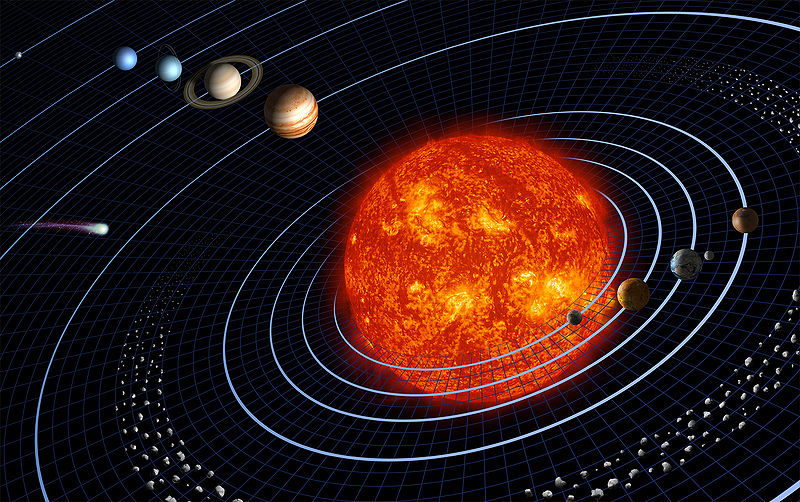
\includegraphics[scale=0.35]{images/solarSis}
        \caption{Sistema Solar}
\end{figure}

Esta Memoria tiene por objetivo desarrollar un sistema informático, que compuesto del software e instrumentos de precisión adecuados, permita a la RedSolLac exponer a la comunidad, información respecto de la producción de energía fotovoltaica de Latinoamérica y el Caribe.\\ 
	
Fundación Chile, es una fundación de carácter privado sin fines de lucro, que se dedica a la creación de valor que aporte al desarrollo del país, dentro de sus áreas de desarrollo encontramos la gerencia de Energía y Cambio Climático que a su vez posee un área de Energía Solar. Dentro del área de Energía Solar se encuentran en ejecución, encargado por el Banco Interamericano de Desarrollo (\gloss{bid}), un proyecto para la creación de una red solar para Latinoamérica y el Caribe, (RedSolLac\cite{redSolLac:1}). El objetivo de esta red es generar a corto y mediano plazo una red de coordinación en la región que sea referente en temas de energía solar y que potencie el desarrollo, la investigación y la utilización de la energía fotovoltaica.\\
 
Como una primera etapa del desarrollo de esta comunidad, se encuentra la integración de estaciones de medición instaladas y por instalar en diferentes regiones de Chile, las cuales generarán una importante data que pasará a formar parte de una base de datos de radiación solar. Estos datos deben estar disponible a toda la comunidad de manera abierta para aportar en el desarrollo de estas energías.\\

Durante el desarrollo de esta Memoria, se implementará una estación de medición y se desarrollará un software que permita difundir los datos capturados, así como herramientas que ayuden en la toma de decisiones respecto de la instalación de sistemas productores de energía fotovoltaica a todo nivel de actividad. En los primeros capítulos se abarcarán los alcances de esta memoria y temas introductorios a la energía solar, mientras que en los siguientes capítulos se describe de manera detallada las herramientas desarrolladas y el proceso de implementación. Finalmente se expondrán los resultados de una fase de captura de datos y prueba del sistema.

\chapter{Alcances de la Memoria}
\label{alcansces}

\section{Problema a resolver}

Actualmente Chile no cuenta con plantas de energía solar fotovoltaica conectadas a sus redes centrales de distribucion (SIC\gloss{SIC}, SING\gloss{SING}, SM\gloss{SM}, SA\gloss{SA}), debido a problemas legales y de normativas tecnicas, la mayoria de las plantas solares que generan energia en chile son plantas aisladas o conectadas a sistemas de distribucion privados, como por ejemplo Calama Solar 3\cite{plantaSolar:1}, Subsole\cite{subsole:2,} entre otras.

La Red Solar para Latinoamerica y el Caribe(RedSolLac) tiene por objetivo contribuir al desarrollo y aprovechamiento de la energia solar fotovoltaica. Ello mediante una plataforma de difusión de información, que facilita la cooperación y colaboración mutua de instituciones, empresas, profesionales y personas interesadas.
Para apoyar la construccion de de la plataforma de difucion de RedSolLac, Esta ha encargado el desarrollo de una aplicacion infromatica, que permita exponer de forma grafica informacion de produccion de energia para plantas solares fotovoltaicas, asi como de estaciones de monitoreo meteorologicas, ademas requiere la construccion de una herramienta que le permita calcular costos de construccion y produccion de energia para apoyar en la toma de desiciones respecto de la construccion de nuevas plantas de energia solar.

\begin{figure}[h!]
        \centering
        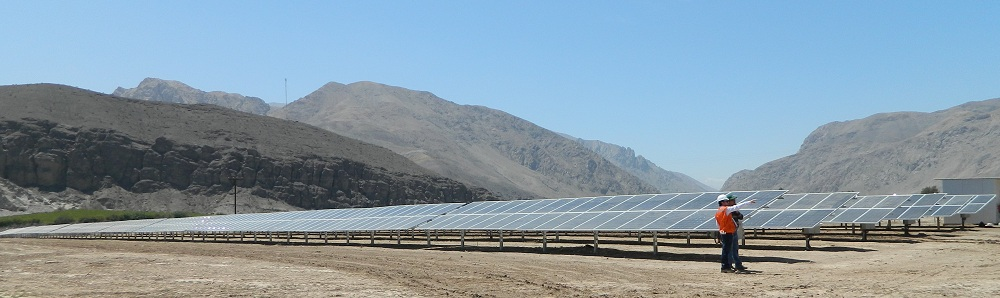
\includegraphics[scale=1.5]{images/plantaSubSoleLorosAmarilla}
        \caption{Planta fotovoltaica 307,2 kWp, sector Los Loros - Tierra Amarilla, región de Atacama - Chile}
\end{figure}
\begin{figure}[h!]
        \centering
        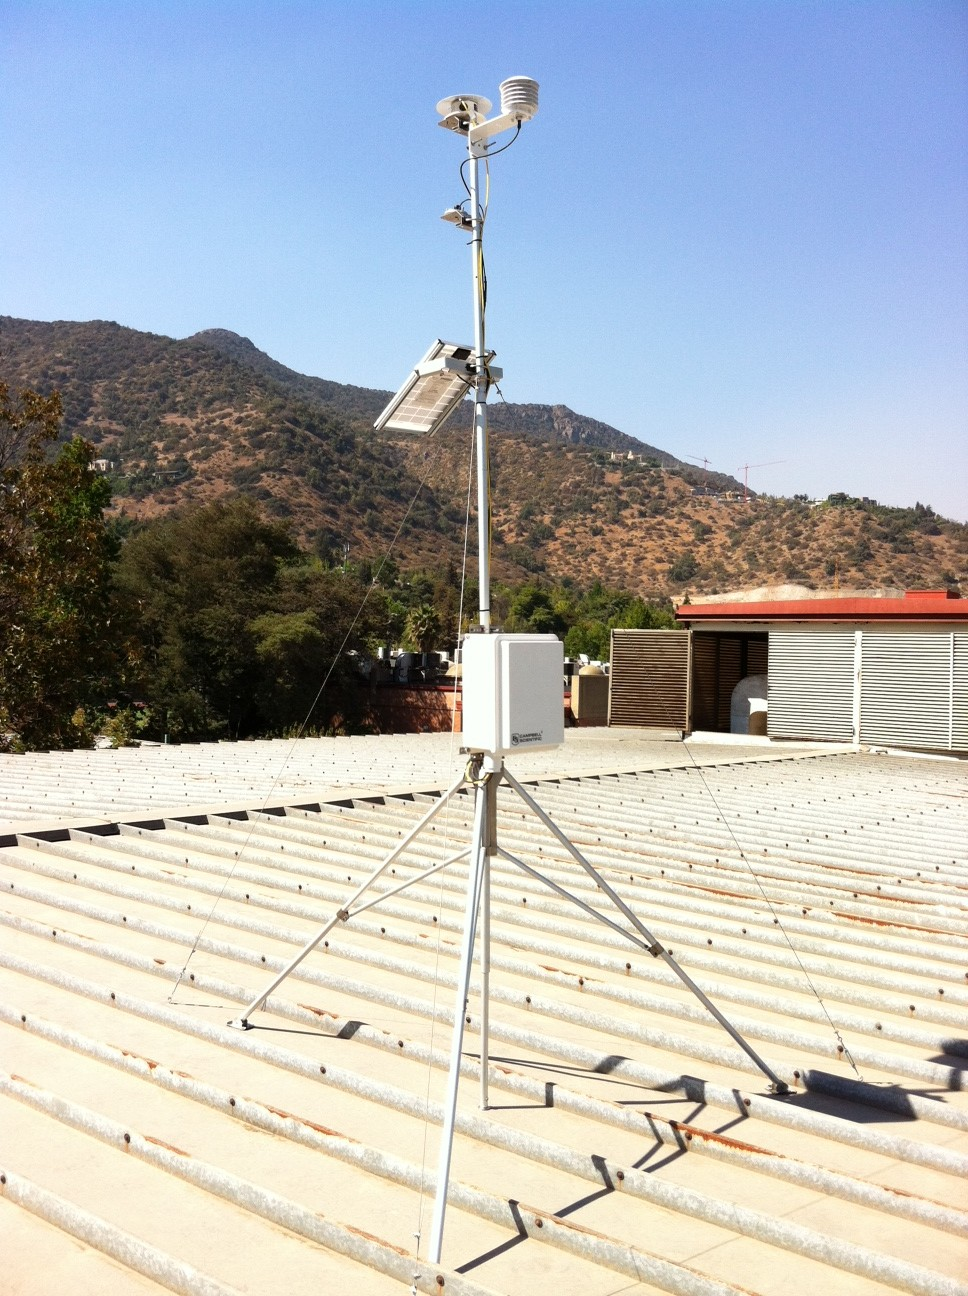
\includegraphics[scale=0.1]{images/estacionMedicionFch}
        \caption{Estación de medición de radiación solar en Fundación Chile, Vitacura - Santiago.}
\end{figure}

Para el desarrollo de este sistema Fundacion Chile utilizara datos de produccion de energia provenientes de diferentes fuentes, entre ellas la nueva planta de Subsole(Fig 2.1), datos de adquisicion propia mediante una estacion meteorologica ubicada en la comuna de Vitacura en la Región Metropolitana(Fig. 2.2) y datos estadisticos publicados por diferentes entidades referentes del tema\cite{datosSolares:1}.

Subsole S.A\cite{subsole:1} es una empresa exportadora de frutas a nivel nacional, a finales del año 2011 finalizo la construccion de una planta solar de 307 kWp\cite{subsole:2} con el objetivo de subministrar corriente elctrica al proceso de riego para la produccion de frutas en el valle de Copiapo en la III Region de Atacama. La planta solar de Subsole es un proyecto pionero para el bombeo de agua mediante el uso de la energía solar para una empresa exportadora de frutas y pretende ser un proyecto modelo para el desarrollo de las ERNC\gloss{ERNC} en los proximos años.\\

El sistema informático actual recibe datos de los inversores y su sistema de medición de energía y almacenamiento de datos, los envía a un sistema privado, el cual no permite la publicación y uso de información, por lo que es necesario implementar un sistema que permita publicar dicha información.\\

\begin{figure}[h!]
        \centering
        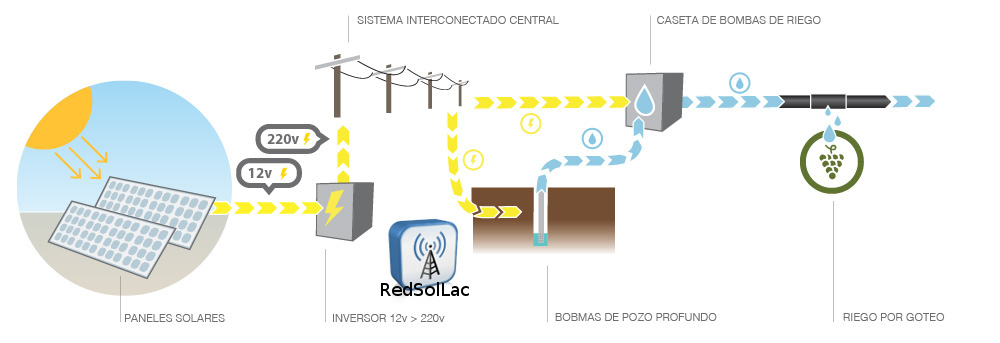
\includegraphics[scale=0.4]{images/plantaSubSoleEsquema}
        \caption{Esquema planta fotovoltaica Subsole 307,2 kWp(STC) a la red eléctrica EMELAT - Región de Atacama}
\end{figure}

La planta eléctrica de Subsole(Fig. 2.3), tiene como objetivo producir suficiente energía que le permita alimentar los motores que extraen el agua de los pozos destinados al riego por goteo. El proyecto original se diseño con la intencion de vender la energia al SIC y que el sistema de riego utilizara al mismo tiempo energia del SIC, actuando la planta como un productor de energia que le permitiria vender o comprar energia dependiendo de la produccion o demanda de esta. Sin embargo esto no se ha podido conretar por dificultades legales, mientras tanto la energia que produce la planta va dirigida directamente al sistema electrico interno.
Los inversores que figuran en el esquema permiten convertir la electricidad producida por los paneles a corriente alterna y 220 Volt, adicionalmente los inversores tienen la capacidad de registrar la información de potencia que pasa por ellos. Dentro del trabajo realizado en esta memoria se contempla instalar un sistema de comunicación para los inversores que permita enviar la información directamente a una base de datos de la RedSolLac en Internet.\\

Ademas se cuenta con una estación de medición de radiación solar, temperatura y humedad ambiente, instalada en Fundación Chile, en la comuna de Vitacura, Santiago de Chile. Esta estacion(Fig. 2.2) en conjunto con la estación meteorológica de la planta fotovoltaica(Fig. 2.3), proporcionarán la información de radiación solar para la calculadora fotovoltaica. Se espera en el futuro incorporar más estaciones de medición.\\

Los principales actores y usuarios de este sistema son todos los miembros de la RedSolLAC, interesados en recibir y compartir información relacionada con la energía solar fotovoltaica. En todo caso la plataforma es abierta por lo que cualquier otro usuario puede acceder a esta información.\\

El BID a través del proyecto RedSolLac que desarrolla la Fundación Chile espera conectar a los actores claves en el desarrollo de la energia solar fotovoltaica de Latinoamérica y el Caribe. En la actualidad, existen pocos actores en la región, por lo que el conocimiento técnico en esta materia se reduce a experiencias de universidades y algunas iniciativas privadas aisladas. La información generada por la planta fotovoltaica Subsole busca convertirse en un sitio de referencia para el estudio y desarrollo de nuevas iniciativas solares.\\

El desarrollo de esta memoria permite la comunidad de la RedSolLac contar con una gran base de datos para ofrecer a todos sus usuarios, así como diversas aplicaciones en su plataforma para la difunción y el patrocinio de la energía solar en la región. Una red como esta potencia el desarrollo de todas las energías renovables no convencionales(ERNC) especialmente la solar fotovoltaica, esto se traduce en un beneficio medioambiental directo para toda la comunidad tanto pertenecientes a la red como a la población en general.

\section{Objetivo principal de la solución}
Desarrollar e implementar un sistema informático para la RedSolLAC que permita interconectar equipos y estaciones de medición solar para la recolección y explotación de datos e información técnica provenientes de una planta solar ubicada en la región de Atacama, Chile.

\section{Objetivos específicos de la solución}
\begin{itemize}
\item Interconectar los diferentes sistemas que componen las estaciones de medición para que exista una comunicación efectiva entre dichos sistemas y una base de datos común en Internet.
\item Desarrollo de un sistema Web capaz de procesar y publicar la información recopilada de una planta de energía solar de gran potencia, ubicada en la región de Atacama.
\item Desarrollo de una calculadora online para sistemas fotovoltaicos, que permita dimensionar y estimar los costos de produccion de energia electrica.
\item Realizar pruebas de la plataforma en conjunto con todos sus componentes, comparar los datos obtenidos con datos recopilados de otras fuentes. Estas prubas permitiran validar el funcionamiento del software asi como la acertividad del metodo de calculo y estimacion electrica implementado en la solución.
\end{itemize}

\section{Requerimientos del sistema}

\subsection{Requerimientos funcionales}
\begin{table}[h!]
\caption{Tabla de requerimientos funcionales}
\begin{tabular}{| c | p{11cm} |}
	\hline
	\textbf{Requerimiento}	&	\textbf{Detalle}	\\
	\hline
	RF-1	&	Registro de datos en linea, las estaciones deben ser programadas para registrar los datos capturados en una base de datos externa en internet, el regisstro de datos debe ser cada 1 minuto.	\\
	\hline
	RF-2	&	La aplicacion debe ser capas de visualizar datos actuales historicos e instantaneos, se debe prporcionar un modulo de visualizacion de datos que permita al usuario visualizar de manera total o parcial los datos registrados por las estaciones, permitiendo seleccionar periodos de tiempo y diferentes tipos de datos proporcionados por los diferentes sensores que conforman la estacion(ver Fig:\ref{fig:demanda}). 	\\
	\hline
	RF-3	&	Descarga de datos, los datos registrados por las estaciones deben estar disponibles para su descarga en un formato practico para la utilizacion de estos por usuarios expertos, pudiendo estos usuarios descargar datos de acuerdo a un periodo de tiempo especificado.	\\
	\hline
	RF-4	&	Permitir el ingreso de informacion, la aplicacion debe permitir el ingreso de parametros geograficos, informacion tecnica de planta y datos economicos para realizar los calculos del dimencionamiento de una planta de energia solar 	\\
	\hline
	RF-5	&	Implementar un modelo de calculo de energia horario basado en el document: ""	\\
	\hline
	RF-6	&	Calcular y exponer resultados de produccion energetica, los resultados deben ser verificables y comparables con otros sistemas, los calculos deben presentar errores no superiroes al 5\%	\\
	\hline
\end{tabular}
\end{table}

\subsection{requerimientos no funcionales}
\begin{table}[h!]
\caption{Tabla de requerimientos no funcionales}
\begin{tabular}{| c | p{11cm} |}
	\hline
	\textbf{Requerimiento}	&	\textbf{Detalle}	\\
	\hline
	RNF-1	&	La aplicacion debe ser independiente del Sistema operativo y del navegador utilizado por el usuarios final	\\
	\hline
	RNF-2	&	Es necesario que la aplicacion se integre con la imagen coorporativa de la RedSolLac	\\
	\hline
	RNF-3	&	El sistema debe entregar estabilidad y muy alta confiabilidad en el registro y amacenamiento de datos	\\
	\hline
	RNF-4	&	La aplicacion debe ser portable y facilmente adaptable para funcionar con multiples fuentes de datos 	\\
	\hline
	RNF-5	&	La aplicacion debe proporcionar un minimo estandar de seguridad que permita asegurar la confiabilidad de los datos	\\
	\hline
	RNF-6	&	La aplicacion debe entregar un resultado al usuario final en tiempo aceptable no mayor a 5 seg	\\
	\hline
\end{tabular}
\end{table}

\begin{figure}[h!]
        \centering
        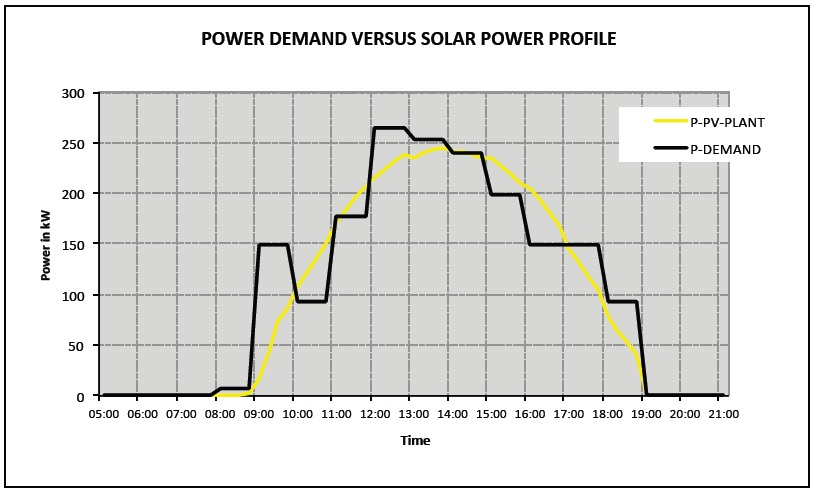
\includegraphics[scale=0.5]{images/demandaGeneracionSubSole}
        \caption{Gráfico de ejemplo de la curva de demanda de energía versus la generación de energía solar fotovoltaica en la planta Subsole.}
	\label{fig:demanda}
\end{figure}

\chapter{Introducción a la energía solar}
\label{solar}

\section{Energías renovables no convencionales}
\subsection{Energía solar térmica}
\subsection{Energía solar fotovoltaica}
\section{Modelo de negocio}
\section{Energía solar en Chile}

\include{chapters/9-Solucion propuesta}
\chapter{Pruebas del sistema}
\label{pruebas}

\section{Funcionamiento del sistema}
\subsection{SolarGraficos}
\subsubsection{Información general de la estación}
\begin{figure}[h]
	\centering
	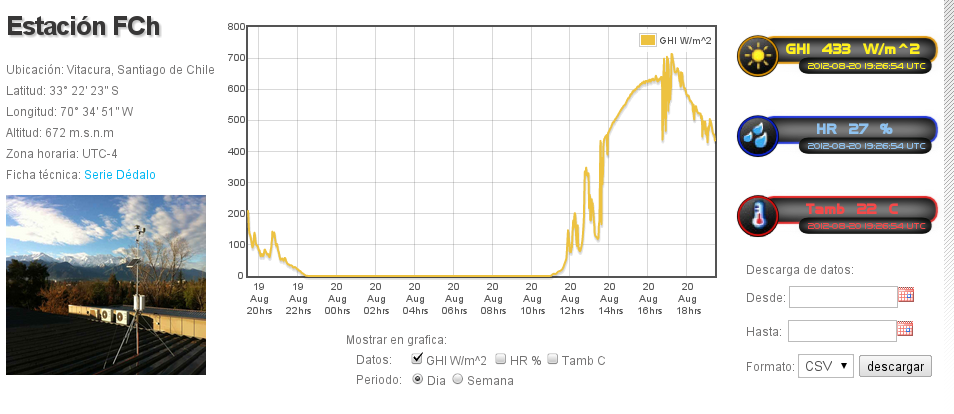
\includegraphics[scale=0.42]{./images/cap5chap1img0}
	\caption{Presentación de la aplicación}
	\label{graficoPresentacion}
\end{figure}
A la izquierda, en la primera columna (Ver. Fig. \ref{graficoPresentacion}), la aplicación muestra la información general de la estación, presentando datos tales como: nombre, ubicación política y geográfica, altitud, zona horaria donde se encuentra y finalmente una ficha técnica sobre el hardware que posee. En la parte inferior se puede apreciar una fotografía de esta.

\begin{figure}[h]
	\begin{minipage}[b]{0.45\linewidth}
		\centering
		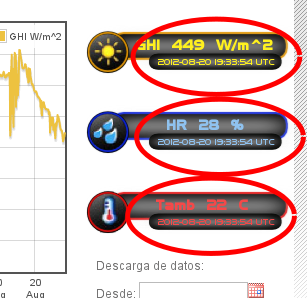
\includegraphics[scale=0.5]{./images/cap5chap1img5-1}
		\caption{Primera marca}
		\label{primeraMarca}
	\end{minipage}
	\begin{minipage}[b]{0.45\linewidth}
		\centering
                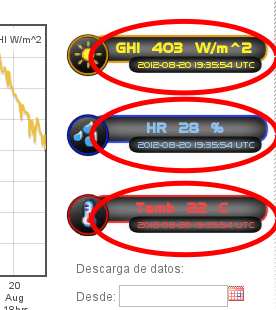
\includegraphics[scale=0.5]{./images/cap5chap1img5-2}
                \caption{Segunda marca}
                \label{segundaMarca}
	\end{minipage}
\end{figure}
En la columna derecha de la aplicación, se presentan indicadores de la ultima medición obtenida (Ver. Fig. \ref{primeraMarca} y \ref{segundaMarca}). Por cada parámetro que la estación mide, hay un ''widget'' que muestra el valor numérico de la medición junto a sus unidades y nombre. En la zona inferior de cada medición se muestra la fecha a la que se asocia dicha medición.

\subsubsection{Manejo del visualizador}
\begin{figure}[ht]
        \centering
        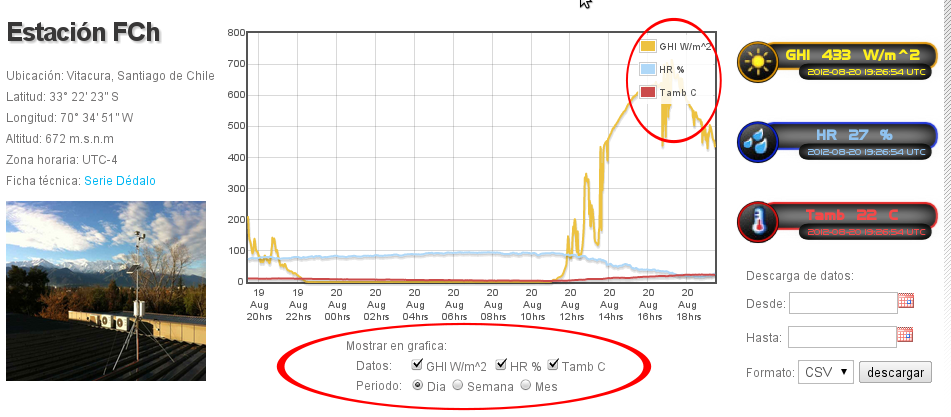
\includegraphics[scale=0.4]{./images/cap5chap1img1}
        \caption{Visualizador - Curvas de la gráfica}
        \label{visualizador}
\end{figure}
La primera herramienta de la cual dispone ''solarGraficos'', da la posibilidad de habilitar o deshabilitar en la gráfica las curvas para los diferentes parámetros medidos por la estación, estas pueden mostrarse de manera individual o bien en conjunto (ver Fig: \ref{visualizador}).

\begin{figure}[ht]
        \centering
        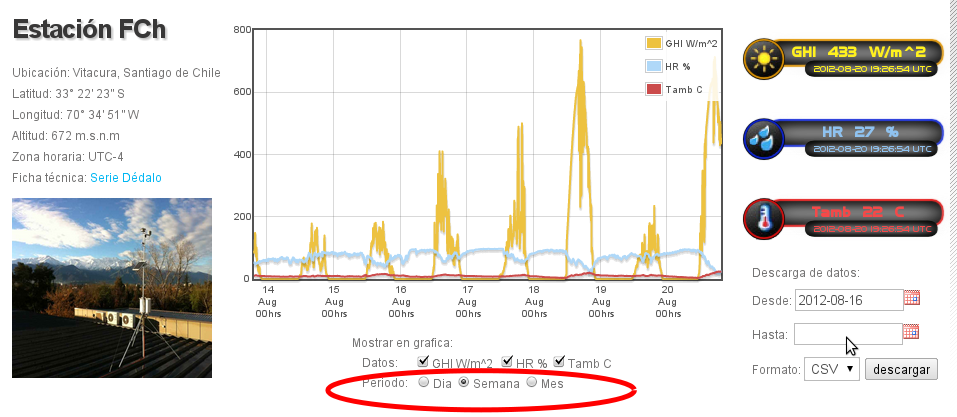
\includegraphics[scale=0.4]{./images/cap5chap1img3}
        \caption{Visualizador - Periodos de tiempo}
        \label{visualizadorTiempo}
\end{figure}
Siguiendo con las herramientas de configuración de la gráfica, la figura \ref{visualizadorTiempo} nos muestra la posibilidad de modificar los periodos de tiempo que se muestran para cada una de las curvas, dado que la cantidad de datos con la que se dibujan las gráficas son bastante grandes, estas toma algún tiempo en cargarse, por lo que si observamos con mas detalle, las opciones para mostrar las curvas en periodos de una semana, un mes o un año, irán apareciendo a medida que los datos estén totalmente cargados. Esta carga ocurre de manera trasparente, por lo que mientras esto sucede el usuario puede hacer uso de todas las demás funcionalidades de la aplicación.\\

Para obtener mas detalles respecto de alguna medición en particular reflejada en la gráfica, basta con posicionar el cursor sobre la curva deseada y esta identificara de manera automática los puntos donde exista una medición, marcando el punto con un circulo a su alrededor, adicionalmente mostrara una pequeña ventana emergente con información detallada de la medición, unidades, hora y fecha especifica. La figura \ref{cursor} muestran como esta característica se aplica a cada una de las curvas.

\begin{figure}[ht]
	\begin{minipage}[b]{0.32\linewidth}
        	\centering
        	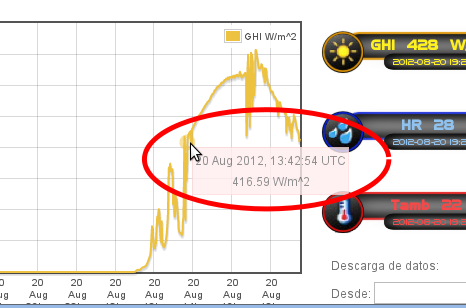
\includegraphics[scale=0.35]{./images/cap5chap1img4-1}
	\end{minipage}
	\begin{minipage}[b]{0.32\linewidth}
                \centering
                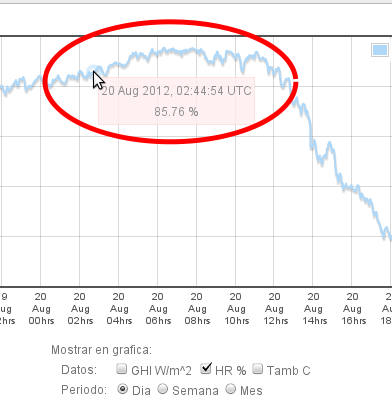
\includegraphics[scale=0.35]{./images/cap5chap1img4-2}
        \end{minipage}
	\begin{minipage}[b]{0.32\linewidth}
                \centering
                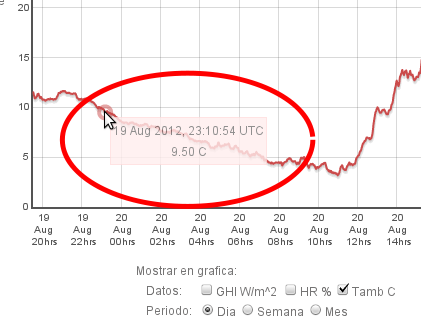
\includegraphics[scale=0.35]{./images/cap5chap1img4-3}
        \end{minipage}
	\caption{Posición del cursor}
	\label{cursor}
\end{figure}

\newpage
\subsubsection{Descarga de datos}
La aplicación cuenta con un módulo que permite descargar los datos directamente desde el ''Servidor de almacenamiento de datos'', de forma personalizada, para ello, en la sección inferior derecha, bajo el titulo ''Descarga de datos'' hay dos campos denominados ''desde'' y ''hasta'', al hacer clic en cada uno de ellos se despliega un calendario que permite seleccionar el día específico para cada campo (Ver. Fig. \ref{calendario}). Mediante esta utilidad podemos especificar el rango de tiempo que contendrá el fichero descargado con los datos en formato CSV. Este fichero puede ser utilizado en diversas aplicaciones externas para cargar los datos y realizar cualquier tipo de procesamiento deseado (Ver. Fig. \ref{descargafichero}).

\begin{figure}[ht]
	\begin{minipage}[b]{0.47\linewidth}
        	\centering
        	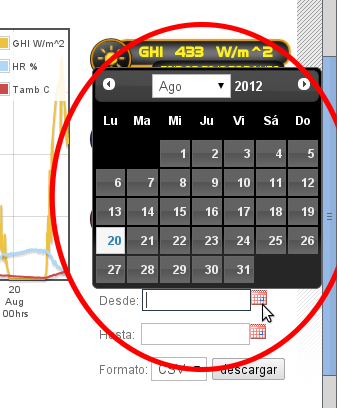
\includegraphics[scale=0.5]{./images/cap5chap1img2-1}
	\end{minipage}
	\begin{minipage}[b]{0.47\linewidth}
	 	\centering
        	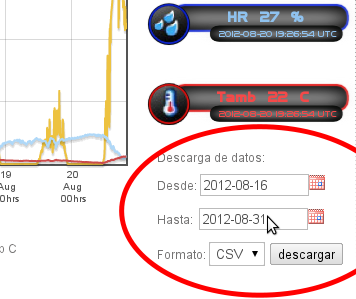
\includegraphics[scale=0.5]{./images/cap5chap1img2-2}
	\end{minipage}
	\caption{Descarga de datos - Calendario}
	\label{calendario}
\end{figure}

\begin{figure}[ht]
	\centering
        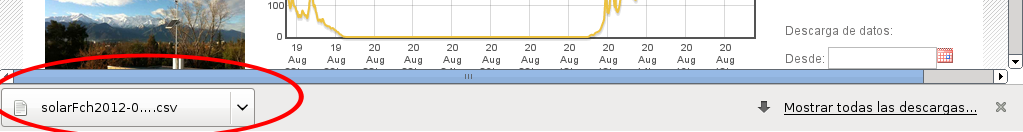
\includegraphics[scale=0.45]{./images/cap5chap1img2-3}
        \label{descargafichero}
	\caption{Descarga de datos - Fichero}
\end{figure}

\newpage 
\subsection{SolarCalc}
\subsubsection{Presentación inicial}
\begin{figure}[ht]
        \centering
        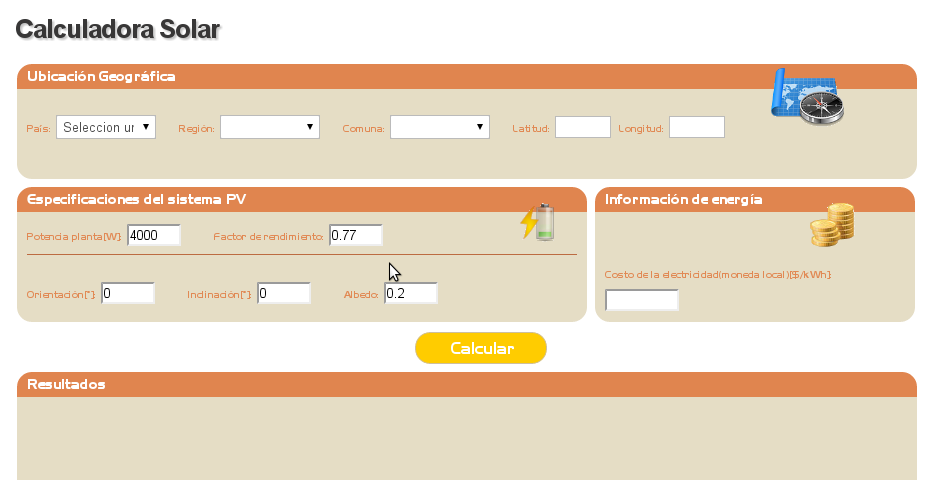
\includegraphics[scale=0.4]{./images/cap5chap1img6}
        \caption{Presentación Calculadora}
        \label{figCalculadora}
\end{figure}

Al cargar la calculadora se aprecia la figura \ref{figCalculadora}, adaptada a los requerimientos planteados, es una interfaz sencilla, con la menor cantidad de parámetros necesarios, los cuales se van actualizando a medida que el usuario los rellena. Dividida en 4 secciones de acuerdo a la caracterización de los parámetros.

\subsubsection{Ubicación geográfica}
La primera sección que se debe rellenar es la posición geográfica donde se pretende instalar la planta a simular, por el momento la calculadora solo cuenta con información de Chile (Ver. Fig. \ref{pais}) en todas sus Regiones y Comunas.\\ Al momento de seleccionar la comuna (Ver. Fig. \ref{region}), el sistema automáticamente establece las coordenadas geográficas del centro de esta. Como indica la figura, los parámetros deben ser ingresados en orden secuencial, iniciando por el país, luego la región y finalmente la comuna, de manera de permitir al sistema ir cargando la información de forma dinámica.
\begin{figure}[ht]
	\centering
	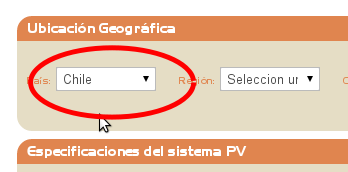
\includegraphics[scale=0.5]{./images/cap5chap1img7-1}
	\caption{País}
	\label{pais}
\end{figure}

\begin{figure}[ht]
	\centering
	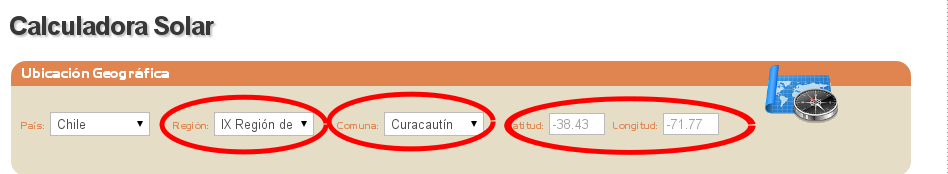
\includegraphics[scale=0.5]{./images/cap5chap1img7-2}
	\caption{Región, comuna, coordenadas geográficas}
	\label{region}
\end{figure}

\subsubsection{Especificaciones del sistema PV e información de la energía}
Esta sección es una de las mas complejas si no se cuenta con cierto conocimiento técnico de los sistemas fotovoltaicos, acá se debe proporcionar a la calculadora parámetros específicos (Ver Fig:\ref{sistemaPv}) de la configuración de los equipos de la planta a simular.\\

\begin{figure}[h]
        \centering
        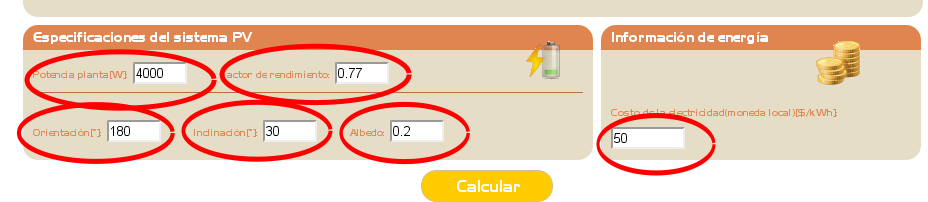
\includegraphics[scale=0.4]{./images/cap5chap1img8}
        \caption{Especificación del sistema PV}
        \label{sistemaPv}
\end{figure}

\paragraph{Potencia de la planta:} Es la suma de la potencia individual de cada uno de los módulos fotovoltaicos del sistema, la que se puede encontrar en la etiqueta trasera de estos.\\
Como referencia, un módulo PV de 1,5[m] de alto por 1[m] de ancho (1,5[m2]) de Silicio policristalino, produce 200[W] de Potencia bajo STC (“Standard Test Conditions” asume 1000[W/m2] de radiación solar, una temperatura ambiente de $25^\circ C$ y velocidad del viento de 1[m/s]).\\ Una instalación de 4000[W] corresponde a 30 [m2] de superficie cubierta con módulos solares.
 
\paragraph{Factor de rendimiento:} Factor que incorpora las pérdidas respecto al proceso completo de conversión de energía, desde que sale de los paneles hasta que está disponible en corriente alterna, respecto a la situación ideal sin pérdidas. Su valor típico es 0.77, variando según el sistema entre 0.62 y 0.96.\\
Consiste en la multiplicación de los factores asociados a pérdidas en los cables, conexiones y diodos, eficiencia del inversor y transformador, variación respecto al valor de placa del módulo solar, entre otros.

\paragraph{Orientación:} Corresponde a la orientación de los paneles respecto al punto cardinal Norte, en la figura expresado por el ángulo $\alpha$ en grados.\\Si el panel se encuentra orientado hacia el Norte, corresponde a $0\circ$, aumentando a medida que se gira hacia el Sur, en sentido horario (Oeste=$270\circ$, Sur=$180\circ$, Este=$90\circ$).

\paragraph{Inclinación:} Corresponde a la inclinación de los paneles respecto al eje horizontal, en la figura expresado por el ángulo $\beta$ en grados.

\begin{figure}[h]
        \centering
        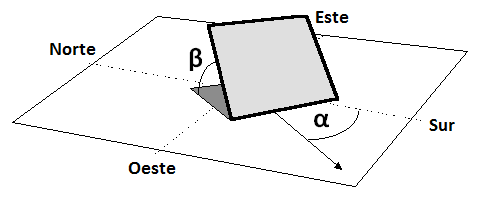
\includegraphics[scale=0.5]{./images/planoPanelSolar}
        \caption{Orientación del sistema PV}
        \label{orientacionSistemaPV}
\end{figure}

\paragraph{Albedo:} Índice sobre el porcentaje de radiación que una superficie refleja, respecto a la que recibe. Mientras mayor es el índice, más radiación refleja. Para el suelo común y corriente se considera 0.2, y para el concreto 0.5, mientras que para la nieve sería 0.85.

\paragraph{Costo de la energía:} Precio que se paga en la moneda local, por cada kWh consumido en el lugar de la instalación.
Generalmente sale expresado en la factura de electricidad.

\subsubsection{Resultados}
Finalmente, luego de llenar toda la información solicitada, se debe hacer clic en el botón ''calcular'', pasados unos segundos el sistema entregara un resultado dividido en 3 sección principales (Ver Fig:\ref{resultadosCalc}). La primera sección es una tabla de resultados la cual nos informa mes a mes para un año típico, la cantidad de radiación media, la cantidad de energía producida específicamente para los parámetros de configuración ingresados y el costo de venta que debiese tener la energía producida, este ultimo paramentar representa una utilidad en cuanto si se desea utilizar estos cálculos en alguna propuesta económica para la instalación de alguna planta.\\ La según sección nos muestra, en la parte inferior izquierda, un gráfico anual en el tiempo y dos ejes laterales, este gráfico nos informa respecto de la eficiencia que tendrá el sistema PV comparando la curva de radiación con la curva de energía producida.\\ Finalmente el gráfico de la para inferior derecha tiene como objetivo caracterizar la radiación solar en un año meteorológico típico para cada mes, con la cual se realizaron los cálculos.

\begin{figure}[h]
        \centering
        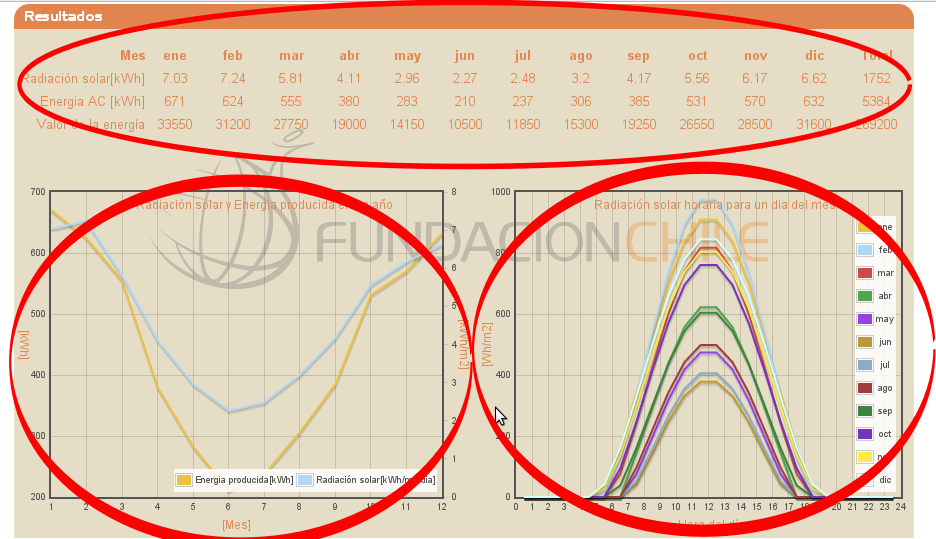
\includegraphics[scale=0.4]{./images/cap5chap1img9}
        \caption{Resultados de la Calculadora}
        \label{resultadosCalc}
\end{figure}

\newpage
\section{Pruebas de comunicación}
Uno de los problemas más complejos que se enfrentó durante el desarrollo de esta Memoria fue el diseño e implementación de los sistemas de comunicación, que permitieron establecer conexiones confiables y seguras entre las distintas componentes del sistema. De acuerdo al diseño planteado en el capítulo \ref{solucion}, se puede apreciar que la comunicación entre la componente de ''Aplicaciones'' y la de ''Almacenamiento de datos'' fue más o menos trivial, dentro de lo que se refiere a la comunicación Web en un sistema informático, sin embargo, al momento de interconectar las ''Estaciones de medición'' con el resto del sistema hubo que considerar muchas variables extras, tales como: geográficas, ambientales y eléctricas.\\

Las estaciones, al estar ubicadas en lugares geográficos remotos, en la mayoría de los casos no disponen de cables o conexiones a la red de datos. La señal de telefonía celular con buen soporte de datos no es de buena calidad en todos los lugares del país y con menor razón en lugares como el Desierto de Atacama, en medio de cordones montañosos e incluso en lugares más aislados. Las estaciones, según requerimientos, debían disponer de un sistema de comunicación flexible, que pudiese ser adaptado a todas las condiciones y dificultades anteriormente mencionadas, para esto se diseño un sistema, de forma que permitiese adaptar diferentes tecnologías, sin embargo, para efectos prácticos de esta Memoria, se implementaron dos módulos diferentes: Comunicación a través de Ethernet y comunicación vía módem de telefonía celular.

\subsection{Caso de Pruebas}
En las próximas secciones de este capitulo se exponen diferentes pruebas realizadas al sistema, entre ellas, la conectividad con las estaciones de medición, los servidores de datos y aplicaciones. Además se realizaron pruebas para verificar los métodos de calculo, la programación y la correctitud de los resultados teóricos en comparación con resultados empíricos. Para las pruebas de comunicación se utilizo una estación Dédalo (Ver Anexo \ref{dedalo}), denominada en capítulos anteriores como ''Estación Fch'' la cual es la estación ubicada en las dependencias de Fundación Chile en la comuna de Vitacura de la Región Metropolitana. Esta estación durante el periodo de prueba midió: Radiación solar global en el plano horizontal, Temperatura ambiente y humedad relativa del aire. Además se considera el periodo de prueba como el funcionamiento normal entre las fechas de Mayo del 2012 y Septiembre 2012, considerando de forma especial una interrupción programada en el mes de Agosto para mantención de los instrumentos, por el periodo de una semana y 6 interrupciones no programadas por fallos en la conectividad del sistema inferiores a 6 horas de funcionamiento cada una, producto del funcionamiento defectuoso de una batería de la estación, lo cual dejo a esta, sin electricidad en dichas ventanas de tiempo, una vez diagnosticado el problema se procedió a reemplazar la batería defectuosa solucionando así el problema.\\
Para la comparación teórica de los cálculos, se utilizaron bases de datos elaboradas por ''PVWatts'', considerando muestras de un año meteorológico típico para la comunas de Vitacura, Antofagasta y Concepción.  
 
\subsection{Comunicación de estación ''VitacuraFCh'' con ''Servidor de datos'' - Vía Ethernet}
Una de las primeras actividades que se realizó en esta Memoria, fue la interiorización con los equipos que componen las estaciones meteorológicas, esto involucró el aprender a utilizar elementos de hardware tales como el ''datalogger'' Campbell Scientific CR1000, módems de telefonía celular y otras interfaces de comunicación.\\
Para lograr que la estación se comunique de forma autónoma con el ''Servidor de almacenamiento de datos'' fue necesario escribir un programa para el ''datalogger'' que fuese capaz de realizar una petición GET a través del módulo ''Campbell NL200'', utilizando la implementación del protocolo TCP/IP de esta Interfaz. Para esto, fue necesario conectar el módulo ''NL200'' a través de la interfaz ''SCI/O'' del ''datalogger'' y configurar el módulo para actuar en modo ''bridge'', esto permite una comunicación transparente, entre el ''datalogger'' y la red informática de Fundación Chile.

Esta modalidad del sistema de comunicación es bastante limitada, ya que es necesario contar en los lugares de instalación de las estaciones con una infraestructura de red de datos informática.

Para verificar el estado de la conexión, se exponen dos métodos, en primer lugar la conexión manual utilizando el software proporcionado por el fabricante ''PC400'', a través de este software establecemos una conexión ''TCP/IP'', utilizando la dirección IP asignada a la estación y realizamos una prueba de descarga de datos:

\begin{enumerate}
\item Ejecutar el PC400
\item Creamos una nueva conexión (Ver Fig:\ref{ether1}) 
\item En la sección ''comunication setup'', seleccionamos el dispositivo ''CR1000'' y luego seleccionamos el tipo de convección ''Ip Port''.
\item Ingresamos la dirección IP de la estación y finalizamos la configuración (Ver Fig:\ref{ether2}).
\item En la pantalla principal, en el menú de la izquierda seleccionamos la nueva interfaz y presionamos el botón ''connect'' (Ver Fig:\ref{ether3})
\item Una vez establecida la conexión, vamos a la solapa superior que dice ''monitor data'' y podemos observar los parámetros que la estación esta midiendo (Ver Fig:\ref{ether4}).
\item Finalmente vamos a la solapa ''collect data'', presionamos en ''collect'' y esperamos a que se complete la descarga (Ver Fig:\ref{ether5}).
\end{enumerate}

\begin{figure}[h!]
        \centering
        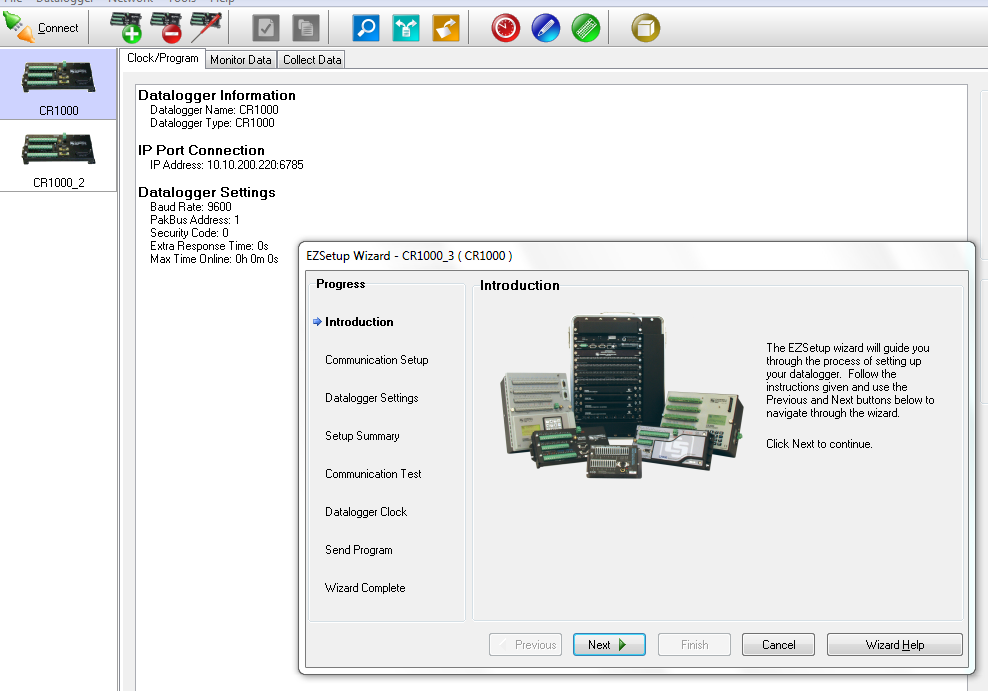
\includegraphics[width=320pt]{images/pruebas1}
        \caption{Crear nueva conexión}
        \label{ether1}
\end{figure}
\begin{figure}[h!]
        \centering
        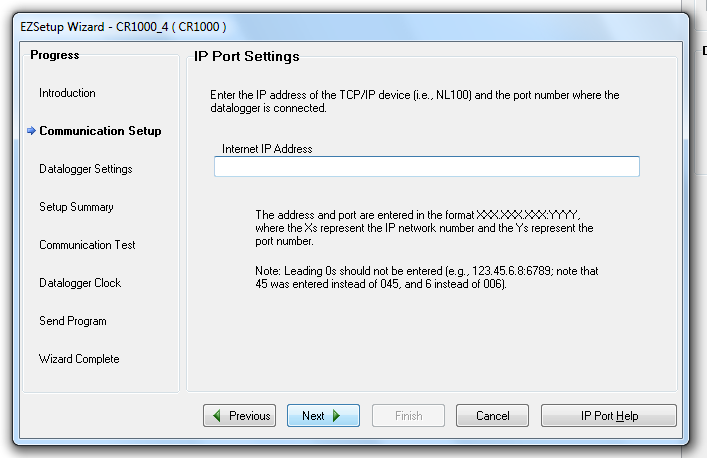
\includegraphics[width=400pt]{images/pruebas2}
        \caption{Ingresar dirección IP}
        \label{ether2}
\end{figure}

\newpage
\begin{figure}[h!]
        \centering
        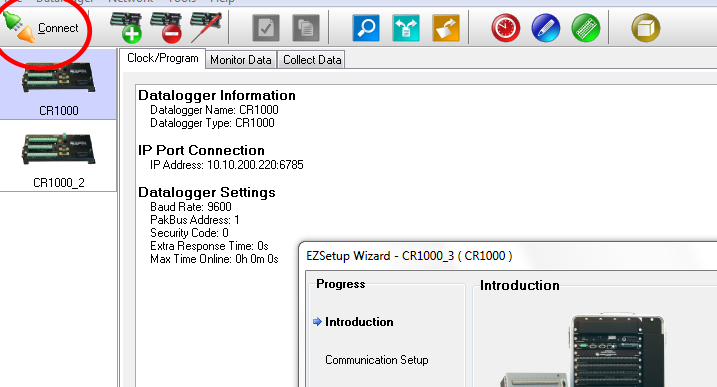
\includegraphics[width=400pt]{images/pruebas3}
        \caption{Estableciendo conexión}
        \label{ether3}
\end{figure}
\begin{figure}[h!]
        \centering
        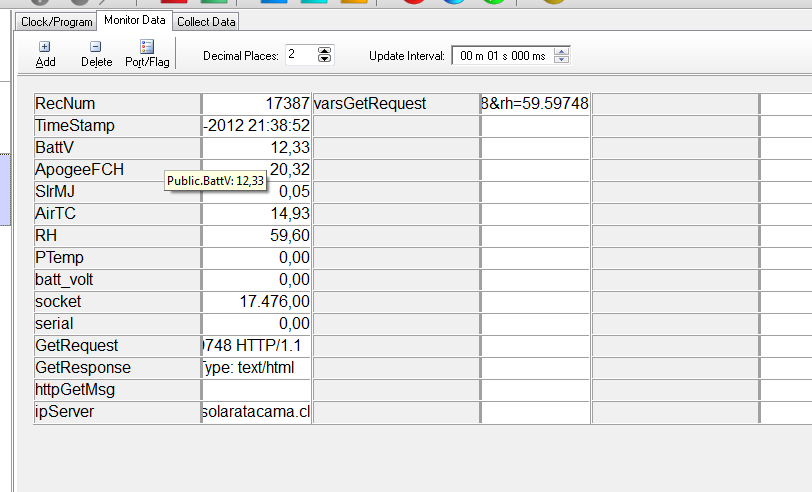
\includegraphics[width=400pt]{images/pruebas4}
        \caption{Monitorizar datos de estación}
        \label{ether4}
\end{figure}

\newpage
\begin{figure}[h!]
        \centering
        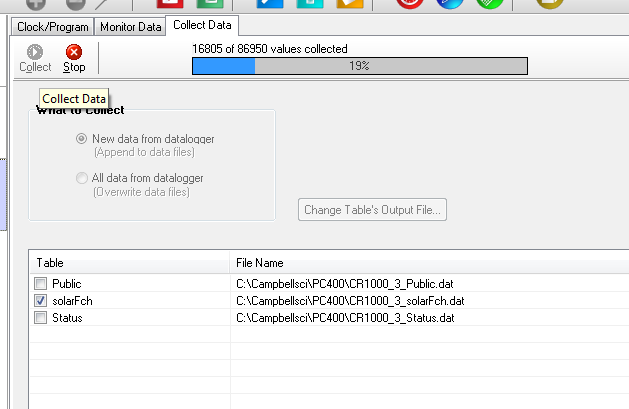
\includegraphics[width=400pt]{images/pruebas5}
        \caption{Descarga de datos}
        \label{ether5}
\end{figure}

\subsection{Comunicación de las estación ''VitacuraFch'' con el ''Servidor de datos''}
Para verificar la conexión autónoma desde la estación hacia la red se presenta el registro del servidor Web Apache HTTPD cuando la estación realiza la petición GET (Ver Fig:\ref{pruebasLog1}).

\begin{figure}[h!]
        \centering
        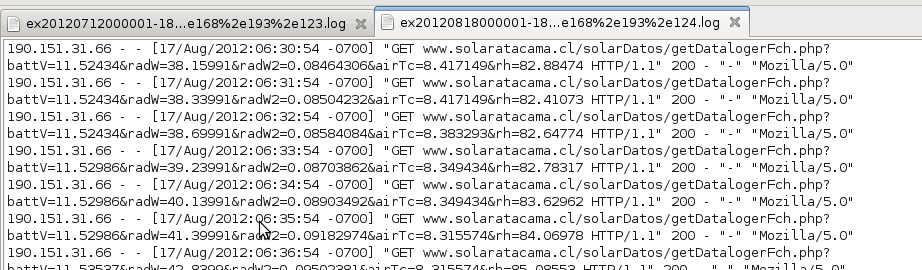
\includegraphics[width=400pt]{images/pruebasLog1}
        \caption{Logs Apache HTTPD - Comunicación con estación meteorológica}
        \label{pruebasLog1}
\end{figure}

\subsection{Comunicación de estación ''VitacuraFCh'' con ''Servidor de datos'' - Vía Módem telefonía celular}
Este tipo de comunicación, es el segundo método que se implementó en esta Memoria y en comparación al método anterior es mucho mas flexible, ya que es posible establecer comunicación con estaciones de forma inalámbrica en diferentes ubicaciones de la geografía nacional, incluso en lugares remotos. Actualmente el desarrollo de esta tecnología en nuestro país, permite establecer comunicación en lugares bastante remotos como sectores montañosos en la cordillera o bien en medio del Desierto de Atacama.\\

Para testear la comunicación mediante este modulo se utiliza el software proporcionado por el fabricante del ''datalogger'', el ''PC400'' siguiendo los siguientes pasos:

\begin{enumerate}
\item Ejecutar el PC400
\item Creamos una nueva conexión (Ver Fig:\ref{ether1})
\item En la sección ''comunication setup'', seleccionamos el dispositivo ''CR800'' y luego seleccionamos el tipo de conexión ''Phone Modem'' (Ver Fig:\ref{modem1}) y luego la opción ''Use módem from CSI list'' (Ver Fig:\ref{modem2}).
\item Seleccionamos el puerto COM donde esta conectado el módem (Ver Fig:\ref{modem3}) y en la lista siguiente, seleccionamos el modelo del miden que vamos a utilizar, Para este caso particular fue necesario configurar un nuevo módem).
\subitem Para configurar un nuevo módem, hacemos clic en ''Edit Modem Database'' (Ver Fig:\ref{modem4}), luego bajo la lista que hay en la nueva ventana desplegada hacemos clic en ''New'', ingresamos el nombre del nuevo módem y presionamos ''OK''
\subitem Finalmente editamos los parámetros del nuevo módem. ''Reset string'' lo seteamos en blanco e ''Initialization String'' lo dejamos en \textbf{\&C0\&D0}, luego hacemos clic en ''Save'' (Ver Fig:\ref{modem5}). 
\item Una vez configurado el módem, ingresamos el ''Phone Number'', numero de teléfono que tienen el módem al cual vamos a llamar y presionamos en ''Next'' para ir al siguiente paso.
\item En esta nueva ventana configuramos el ''Baud Rate'' en \textbf{9600} y Finalizamos la configuración.
\item Finalmente hacemos clic en el botón superior izquierdo con la nueva conexión seleccionada para abrir un canal de comunicación con la estación.
\item Una vez establecida la conexión vamos a la solapa superior que dice ''monitor data'' y podemos observar los parámetros que la estación esta midiendo (Ver Fig:\ref{ether4}).
\item Finalmente vamos a la solapa ''collect data'', presionamos en ''collect'' y esperamos a que se complete la descarga (Ver Fig:\ref{ether5}).
\end{enumerate}
\begin{figure}[h!]
        \centering
        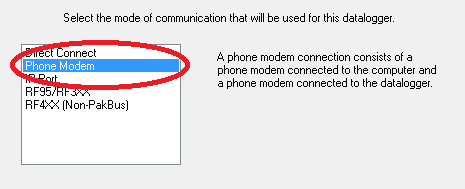
\includegraphics[width=320pt]{images/modem1}
        \caption{Seleccionar módem}
        \label{modem1}
\end{figure}
\begin{figure}[h!]
        \centering
        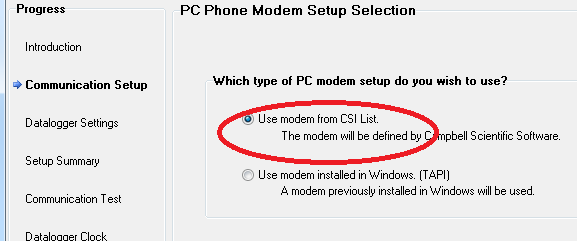
\includegraphics[width=320pt]{images/modem2}
        \caption{Seleccionar puerto}
        \label{modem2}
\end{figure}
\newpage

\begin{figure}[h!]
        \centering
        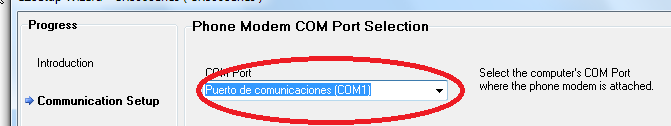
\includegraphics[width=320pt]{images/modem3}
        \caption{Ingresar numero telefónico}
        \label{modem3}
\end{figure}
\begin{figure}[h!]
        \centering
        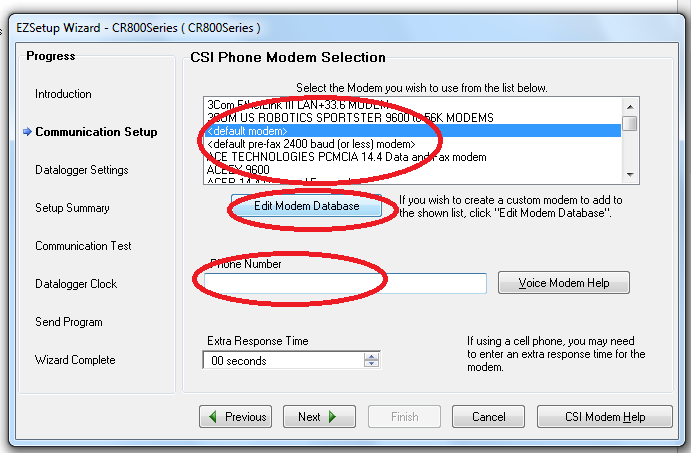
\includegraphics[width=320pt]{images/modem4}
        \caption{Agregar nuevo módem}
        \label{modem4}
\end{figure}

\newpage
\begin{figure}[h!]
        \centering
        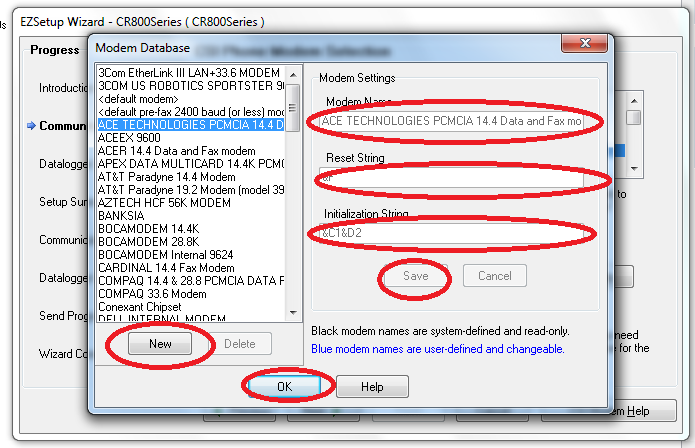
\includegraphics[width=300pt]{images/modem5}
        \caption{Ingresar dirección IP}
        \label{modem5}
\end{figure}

\newpage
\section{Verificación de datos}
Una ves desarrollado el sistema con todas las aplicaciones que cubren los requerimientos planteados en el capitulo \ref{alcances} de esta Memoria, es necesario verificar que los datos obtenidos sean correctos y de la misma forma los cálculos a los que estos son sometidos.\\
Ha quedado expresado en la sección de requerimientos que la confiabilidad de los datos así como del proceso de calculo es esencial en el funcionamiento del sistema, pequeños errores en el sistema de calculo podrían significar grandes errores en el dimensionamiento de los sistemas fotovoltaicos, lo que podría traer consecuencias poco deseables a los actores de la RedSolLAC.\\
Es necesario recordar que durante el desarrollo de esta Memoria se implementó un nuevo método de calculo, que intenta mejorar sistemas anteriores, por lo que es sumamente necesario comprobar y exponer las diferencias en los resultados obtenidos, así como de resaltar las mejoras que este método propone.\\

Los resultados obtenidos fueron comparados con diferentes fuentes de datos, así como con diferentes modelos de cálculos, algunos de ellos, los mas relevantes, son presentados a continuación junto con el análisis correspondiente a las diferencias encontradas.\\
La primera verificación apunta a comprobar que el modelo matemático haya sido bien implementado, luego se presentan 3 resultados obtenidos con la calculadora desarrollada y 2 sistemas externos, finalmente comparamos los resultados teóricos con los obtenidos en un sistema PV en operación.\\

\subsection{PVWatts}
A la fecha de desarrollo de esta Memoria, es el único software en formato Web existente, que ofrece el servicio de calculo y dimensionamiento de sistemas fotovoltaicos que cuenta con información para algunas localidades en Latinoamérica. Sin embargo en su método de calculo implementa un modelo basado en la ''media de la radiación mensual'', como consecuencia de esto, entrega resultados notablemente inferiores al real.\\ 
\subsection{PVSyst}
Es un software privativo, de uso profesional para el sector de la industria energética solar. Este software permite diseñar, estudiar, dimensionar y simular sistemas fotovoltaicos, con un método de calculo bastante complejo y cercano al funcionamiento real de una planta solar fotovoltaica, considerando complejas variables que influyen en el calculo, tales como el sombreado producido por los mimos módulos del sistema o la sombra generada por cerros cercanos a las instalaciones.\\

\subsection{Comparación ''solarCalc'' con ''Plataforma Web para sistemas térmicos''}
La ''Plataforma Web para sistemas térmicos (Ver Anexo \ref{memoriaEdu2})'' es una de las bases con las cuales se implemento el sistema de calculo. Para el proceso de verificación se utiliza una ''macro en excel'' originada en dicho trabajo y los resultados entregados en modo de depuración por la calculadora.\\
Mediante este método se pretende verificar que la implementación de la calculadora sea correcta y entregue los valores esperados.

\begin{landscape}
\begin{table}[h!]
\caption{Resultados verificación de ecuaciones macro excel}
\label{excel}
\resizebox{22cm}{!}{
\begin{tabular}{|l|c|c|c|c|c|c|c|c|c|c|c|c|c|c|c|c|c|c|c|c|c|c|c|c|c|}
        \hline
        \textbf{Resultados macro excel}&&&&&&&&&&&&&&&&&&&&&&&&&\\
        \hline
        \textbf{Hora del día}&0.5&1.5&2.5&3.5&4.5&5.5&6.5&7.5&8.5&9.5&10.5&11.5&12.5&13.5&14.5&15.5&16.5&17.5&18.5&19.5&20.5&21.5&22.5&23.5&Total\\
        \hline
        \textbf{Radiación Global Horizontal horaria}&0&0&0&0&0&20.6&203.3&421.1&650.8&862.4&1025.2&1113.7&1113.7&1025.2&862.4&650.8&421.1&203.3&20.6&0&0&0&0&0&8594.2\\
        \hline
        \textbf{Radiación Difusa Horizontal horaria}&0&0&0&0&0&5.9&51.5&95.6&135.1&167.4&190.2&202&202&190.2&167.4&135.1&95.6&51.5&5.9&0&0&0&0&0&1695.4\\
        \hline
        \textbf{Radiación Directa Horizontal horaria}&0&0&0&0&0&14.7&151.8&325.5&515.7&695.1&835&911.7&911.7&835&695.1&515.7&325.5&151.8&14.7&0&0&0&0&0&6899\\
        \hline
\end{tabular}
}
\end{table}

\begin{table}[h!]
\caption{Resultados verificación de ecuaciones calculadora}
\label{ecuacionCalc}
\resizebox{22cm}{!}{
\begin{tabular}{|l|c|c|c|c|c|c|c|c|c|c|c|c|c|c|c|c|c|c|c|c|c|c|c|c|c|}
        \hline
        \textbf{Resultados macro excel}&&&&&&&&&&&&&&&&&&&&&&&&&\\
        \hline
        \textbf{Hora del día}&0.5&1.5&2.5&3.5&4.5&5.5&6.5&7.5&8.5&9.5&10.5&11.5&12.5&13.5&14.5&15.5&16.5&17.5&18.5&19.5&20.5&21.5&22.5&23.5&Total\\
        \hline
        \textbf{Radiación Global Horizontal horaria}&0&0&0&0&0&21&204&421&651&862&1025&1114&1114&1025&862&651&421&204&21&0&0&0&0&0&8596\\
        \hline
        \textbf{Radiación Difusa Horizontal horaria}&0&0&0&0&0&6&52&96&135&167&190&202&202&190&167&135&96&52&6&0&0&0&0&0&1696\\
        \hline
        \textbf{Radiación Directa Horizontal horaria}&0&0&0&0&0&15&152&325&516&695&835&912&912&835&695&516&325&152&15&0&0&0&0&0&6900\\
        \hline
\end{tabular}
}
\end{table}
\end{landscape}

\newpage
Como se puede apreciar en las tablas \ref{excel} y \ref{ecuacionCalc} la pequeña diferencia obtenida en los resultados, solo atienden a una diferencia de aproximación numérica, mas haya de eso, los números verifican que el modelo de calculo ha quedado implementado correctamente.

\subsection{''solarCalc'' v/s ''PVWatts'' v/s ''PVSist con datos de la comuna Antofagasta}
\begin{table}[h!]
\caption{Comparación de software con datos de Antofagasta}
\resizebox{15cm}{!}{
\begin{tabular}{|c|c|c|c|c|}
        \hline
	\textbf{Mes}&\textbf{Antofagasta (kWh/m2/día)}&\textbf{Energía estimada PVWatts (kWh)}&\textbf{Energía estimada solarCalc (kWh)}&\textbf{Energía estimada PVSist (kWh)}\\
	Ene&	7.70&	630&	794&	652\\
        \hline
	Feb&	7.62&	593&	751&	622\\
        \hline
	Mar&	6.71&	642&	797&	686\\
        \hline
	Abr&	5.48&	570&	690&	617\\
        \hline
	May&	4.12&	472&	566&	527\\
        \hline
	Jun&	3.63&	423&	505&	471\\
        \hline
	Jul&	3.75&	444&	528&	492\\
        \hline
	Ago&	4.65&	514&	528&	569\\
        \hline
	Sep&	5.68&	556&	676&	595\\
        \hline
	Oct&	6.68&	620&	755&	645\\
        \hline
	Nov&	6.96&	578&	710&	579\\
        \hline
	Dic&	7.63&	620&	777&	636\\
        \hline
	Total&5.87&	6662&	8172&	7089\\
        \hline
\end{tabular}
}
\end{table}
Tal como se aprecia en la tabla de datos, los resultados obtenidos por la ''solarCalc'' son notoriamente mas elevados que ambos sistemas, un $18\%$ mas que ''PVWatts'' y un $13\%$ mas que ''PVSyst'' estos son resultados esperados, en primer lugar, la primera diferencia se supone debido a la mejora con el método de calculo propuesto, la segunda diferencia si bien sigue siendo elevada es ligeramente menor esto se explica debido a que la calculadora a pesar de que mejora el método de calculo acercandoce mas al ideal de ''PVSyst'' no considera un parámetro sumamente importante como lo es la disminución en rendimiento por causa de la temperatura ambiente, la cual produce una significativa disminución de la producción cuando estas son elevadas como se puede espera de la zona norte de Chile.

\newpage
\subsection{''solarCalc'' v/s ''PVWatts'' v/s ''PVSist con datos de Vitacura}
\begin{table}[h!]
\caption{Comparación de software con datos de Vitacura}
\resizebox{15cm}{!}{
\begin{tabular}{|c|c|c|c|c|}
        \hline
	\textbf{Mes}&\textbf{Vitacura (kWh/m2/día)}&\textbf{Energía estimada Pivotas (kW)}&\textbf{Energía estimada solarCalc (kWh)}&\textbf{Energía estimada PVSist (kWh)}\\
	Ene&	7.6&	641&	778&	609\\
        \hline
	Feb&	7.45&	563&	751&	609\\
        \hline
	Mar&	6.39&	550&	811&	684\\
        \hline
	Abr&	4.69&	393&	665&	595\\
        \hline
	May&	3.29&	288&	537&	516\\
        \hline
	Jun&	2.75&	233&	469&	440\\
        \hline
	Jul&	2.77&	245&	464&	434\\
        \hline
	Ago&	3.81&	340&	576&	539\\
        \hline
	Sep&	4.74&	407&	604&	526\\
        \hline
	Oct&	5.6&	492&	648&	545\\
        \hline
	Nov&	7.11&	592&	725&	583\\
        \hline
	Dic&	7.09&	600&	716&	592\\
        \hline
	Total&	5.26&	5344&	7744&	6673\\
        \hline
\end{tabular}
}
\end{table}
Al igual que en el caso anterior los resultados apreciados son muy elevados, un $30\%$ mas que ''PVWatts'' y un $13\%$ mas que ''PVSyst''. la diferencia excesiva con de la primera cifra se explica debido a que el nuevo método de calculo considera parámetros como la latitud el cual afectan notoriamente de acuerdo a la posición del sol. En el segundo resultado observamos que la diferencia se mantiene con el caso de Antofagasta lo que representa una buena señal al mantener el mismo porcentaje de diferencia.

\newpage
\subsection{''solarCalc'' v/s ''PVWatts'' v/s ''PVSist con datos de Concepción}
\begin{table}[h!]
\caption{Comparación de software con datos de Concepción}
\resizebox{15cm}{!}{
\begin{tabular}{|c|c|c|c|c|}
        \hline
	\textbf{Mes}&\textbf{Concepción (kWh/m2/día)}&\textbf{Energía estimada PVWatts (kWh)}&\textbf{Energía estimada solarCalc (kWh)}&\textbf{Energía estimada PVSist (kWh)}\\
	Ene&	7.64&	662&	778&	628\\
        \hline
	Feb&	6.81&	574&	751&	603\\
        \hline
	Mar&	4.93&	511&	811&	639\\
        \hline
	Abr&	3.39&	381&	665&	575\\
        \hline
	May&	1.89&	218&	537&	375\\
        \hline
	Jun&	1.54&	180&	469&	327\\
        \hline
	Jul&	1.79&	220&	464&	405\\
        \hline
	Ago&	2.53&	292&	576&	460\\
        \hline
	Sep&	3.97&	422&	604&	557\\
        \hline
	Oct&	5.42&	530&	648&	593\\
        \hline
	Nov&	6.55&	568&	725&	557\\
        \hline
	Dic&	7.54&	641&	716&	597\\
        \hline
	Total&	4.49&	5198&	7744&	6315\\
        \hline
\end{tabular}
}
\end{table}
Finalmente la ultima comparación realizada, es para la comuna de Concepción. Los resultados obtenidos fueron de un $18\%$ para ''PVWatts'' y $0,32\%$ para ''PVSyst''. Analizando estos resultados se puede concluir que son muy favorables ya que en primer lugar mantenemos la mejora con respecto del primer sistema y por otro lado nos acercarnos de manera muy precisa al software de simulación profesional. Lo importante de este resultado es que la comparación con ''PVSyst'' es muy buena y esto se explica ya que en el sur del país las temperaturas promedio durante la hora de funcionamiento de las plantas son notoriamente menores que en Antofagasta y Santiago, esto viene a corroborar la tesis donde se plantea que la corrección por temperatura de la que carece la calculadora afectan significativamente a los cálculos.

\newpage
\subsection{Comparación con sistema PV en operación}
La ultima verificación a la cual se ha sometido la aplicación construida es una verificación empírica. Utilizando un sistema fotovoltaico en operación, se ha obtenido una muestra para el mes de Septiembre 2012, luego esta muestra se ha comparado con la simulación entregada por ''solarCalc'' y por ''PVSyst''. Si bien la muestra obtenida es en un periodo bastante corto como para concluir de manera definitiva sobre la correctitud del sistema, es una muestra que nos da una aproximación respecto de que tan cerca puede estar el resultado teórico con el resultado obtenido en la planta real.\\

\begin{table}[h!]
\caption{Comparación de resultados teóricos v/s empíricos para el mes de Septiembre 2012 (KWh)}
\centering
\begin{tabular}{|c|c|c|}
        \hline
        \textbf{MarceloMena}&\textbf{PVSyst}&\textbf{SolarCalc}\\
        163,4 Kwh&    164,8 Kwh&   190 Kwh\\
        \hline
\end{tabular}
\end{table}

En los resultados obtenidos se pueden apreciar varias cosas, primeramente la similitud de los resultados entre la ''planta solar'' y ''PVSyst'' lo que nos da una idea de lo certera que es esta herramienta para el calculo y dimensionamiento de plantas solares obteniendo aproximadamente un 1\% de diferencia. Por otro lado podemos apreciar el resultado entregado por la calculadora de $190 [kWh]$ lo que representa un 16\% mas de la producción real, si bien el resultado es excesivamente alto, es un resultado sumamente esperado debido a que la calculadora no considera en su sistema de calculo la variabilidad que existe por consecuencia de la baja en el rendimiento por temperatura de operación del sistema PV, si consideramos que esta perdida es aproximadamente de un 10\% se obtienen valores cercanos a 171 Kwh, quedando una diferencia de sobre producción de un 4,65\% con el sistema real.

\chapter{Conclusiones}

\chapter{Anexos}
\label{anexos}

\newpage
\includepdf[scale=0.95,pages={1},offset=3cm 0cm,pagecommand={\section{Memoria Msc. Eduardo Soto}\label{memoriaEdu2}\thispagestyle{empty}}]{include/masterEdu}
\includepdf[scale=0.95,pages={2-9},offset=3cm -1cm]{include/masterEdu}

\newpage
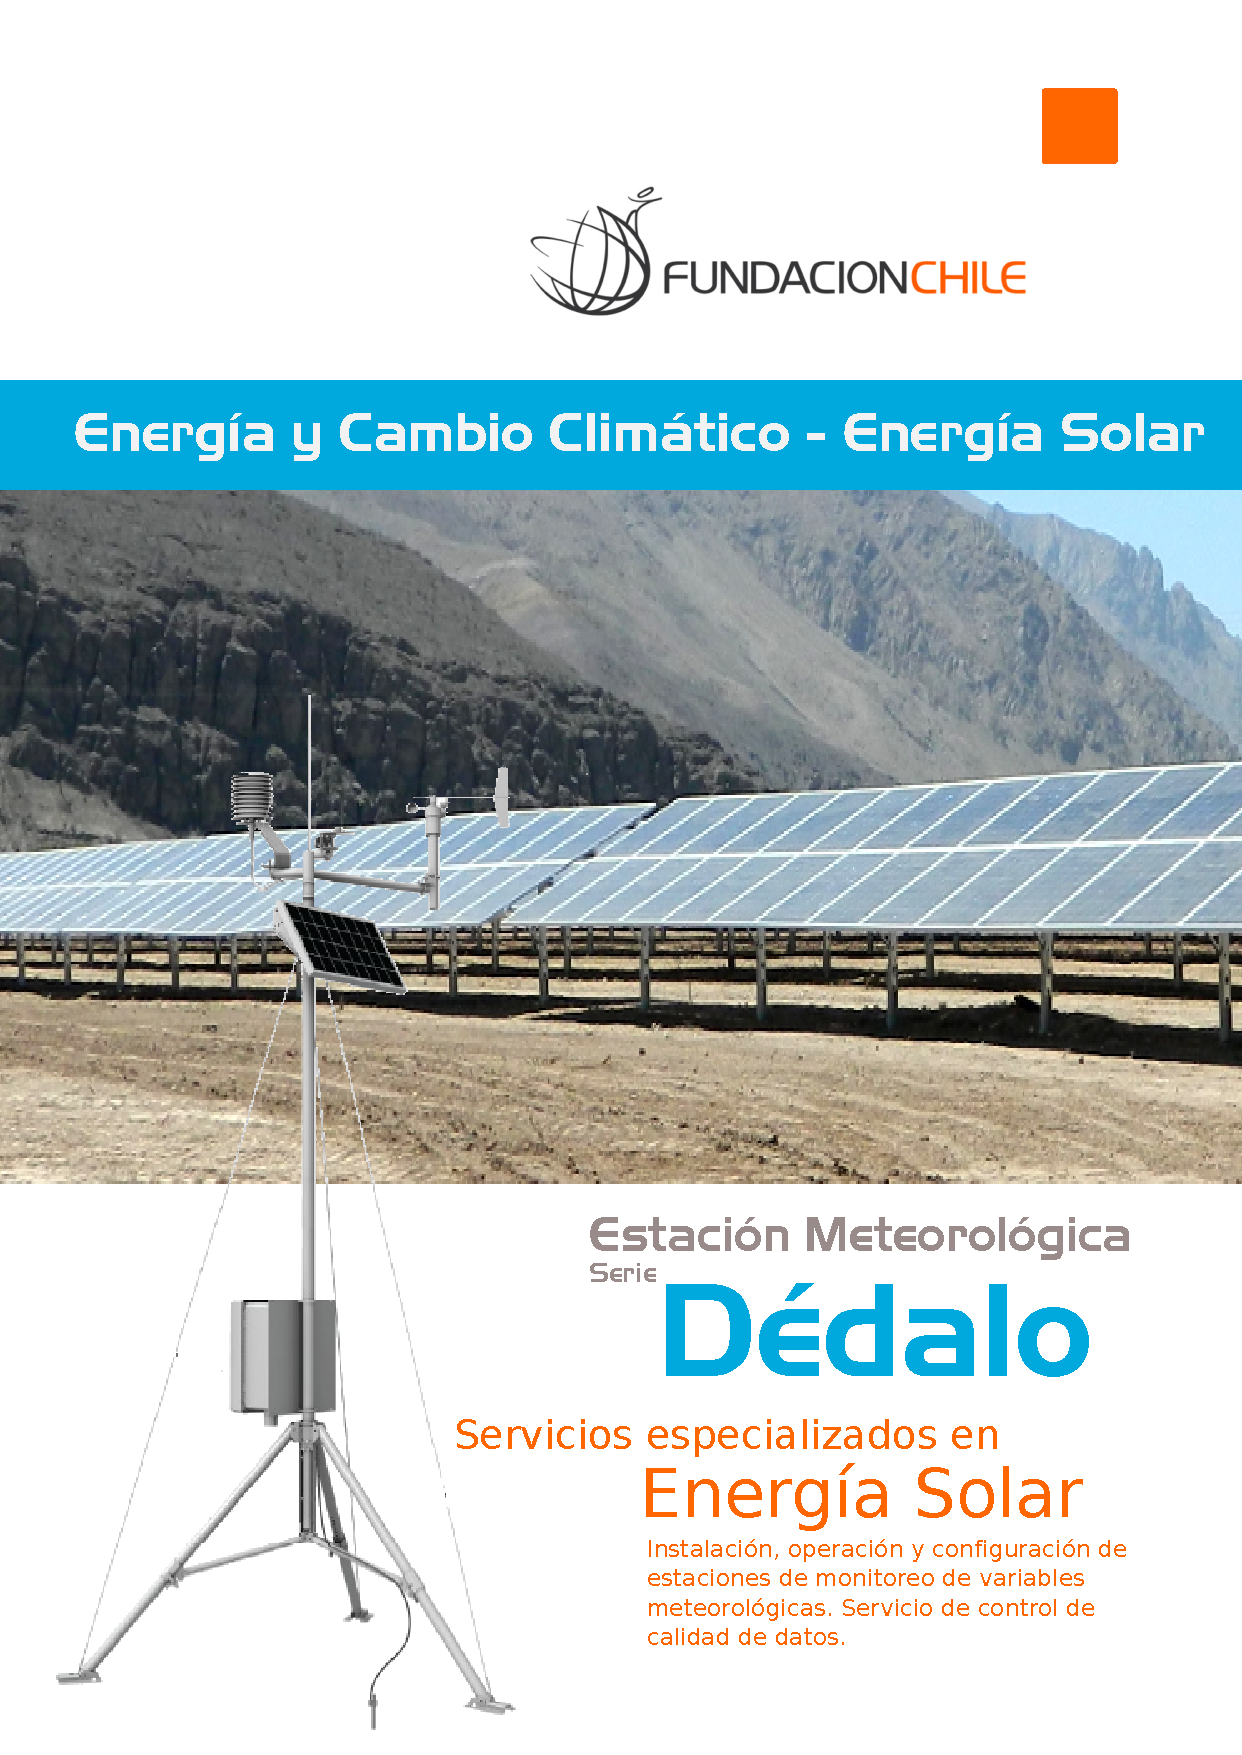
\includepdf[scale=0.95,pages={1},offset=3cm 0cm,pagecommand={\section{Estación serie Dédalo}\label{dedalo}\thispagestyle{empty}}]{include/fichaTecnicaDedalo}
\includepdf[scale=0.95,pages={2-3},offset=3cm -1cm]{include/fichaTecnicaDedalo}

\newpage
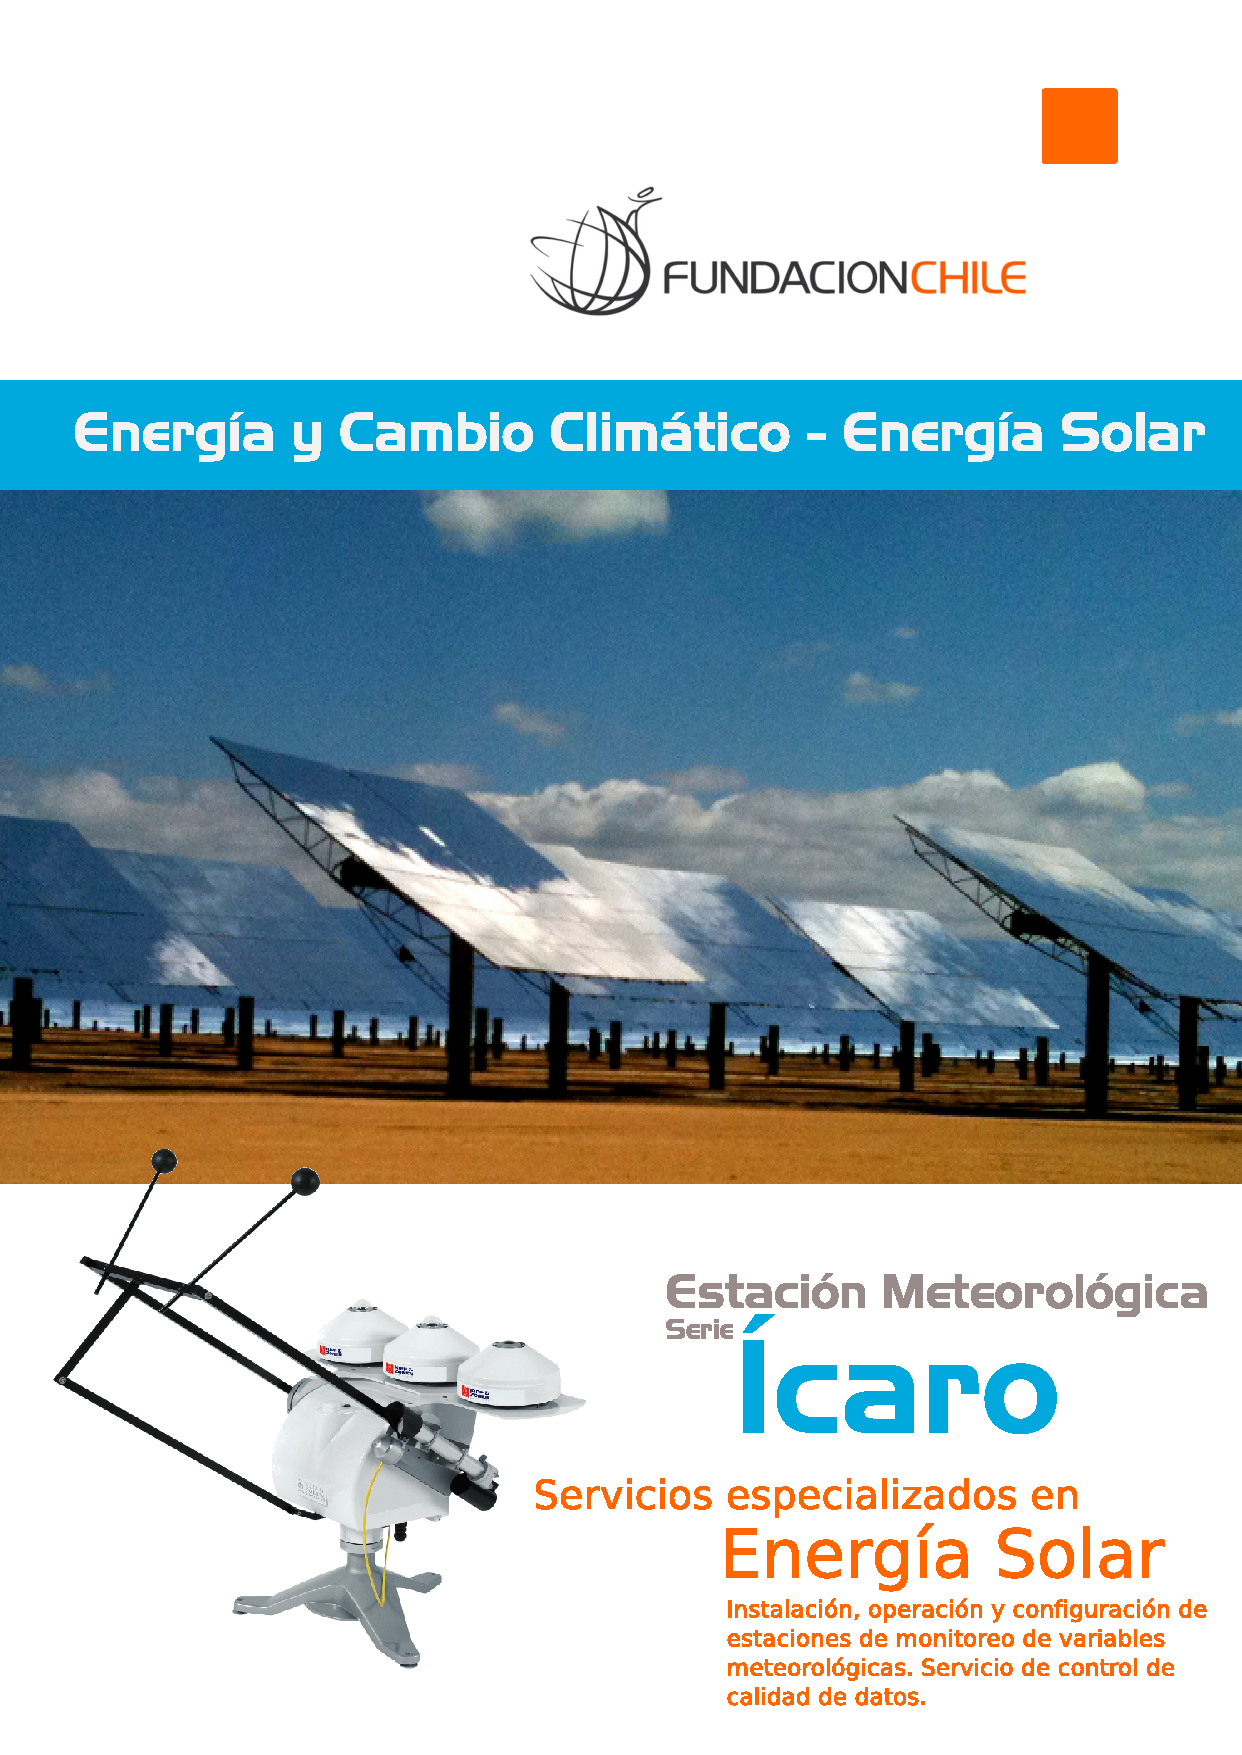
\includepdf[scale=0.95,pages={1},offset=3cm 0cm,pagecommand={\section{Estación serie Ícaro}\label{icaro}\thispagestyle{empty}}]{include/fichaTecnicaIcaro}
\includepdf[scale=0.95,pages={2-3},offset=3cm -1cm]{include/fichaTecnicaIcaro}

\newpage
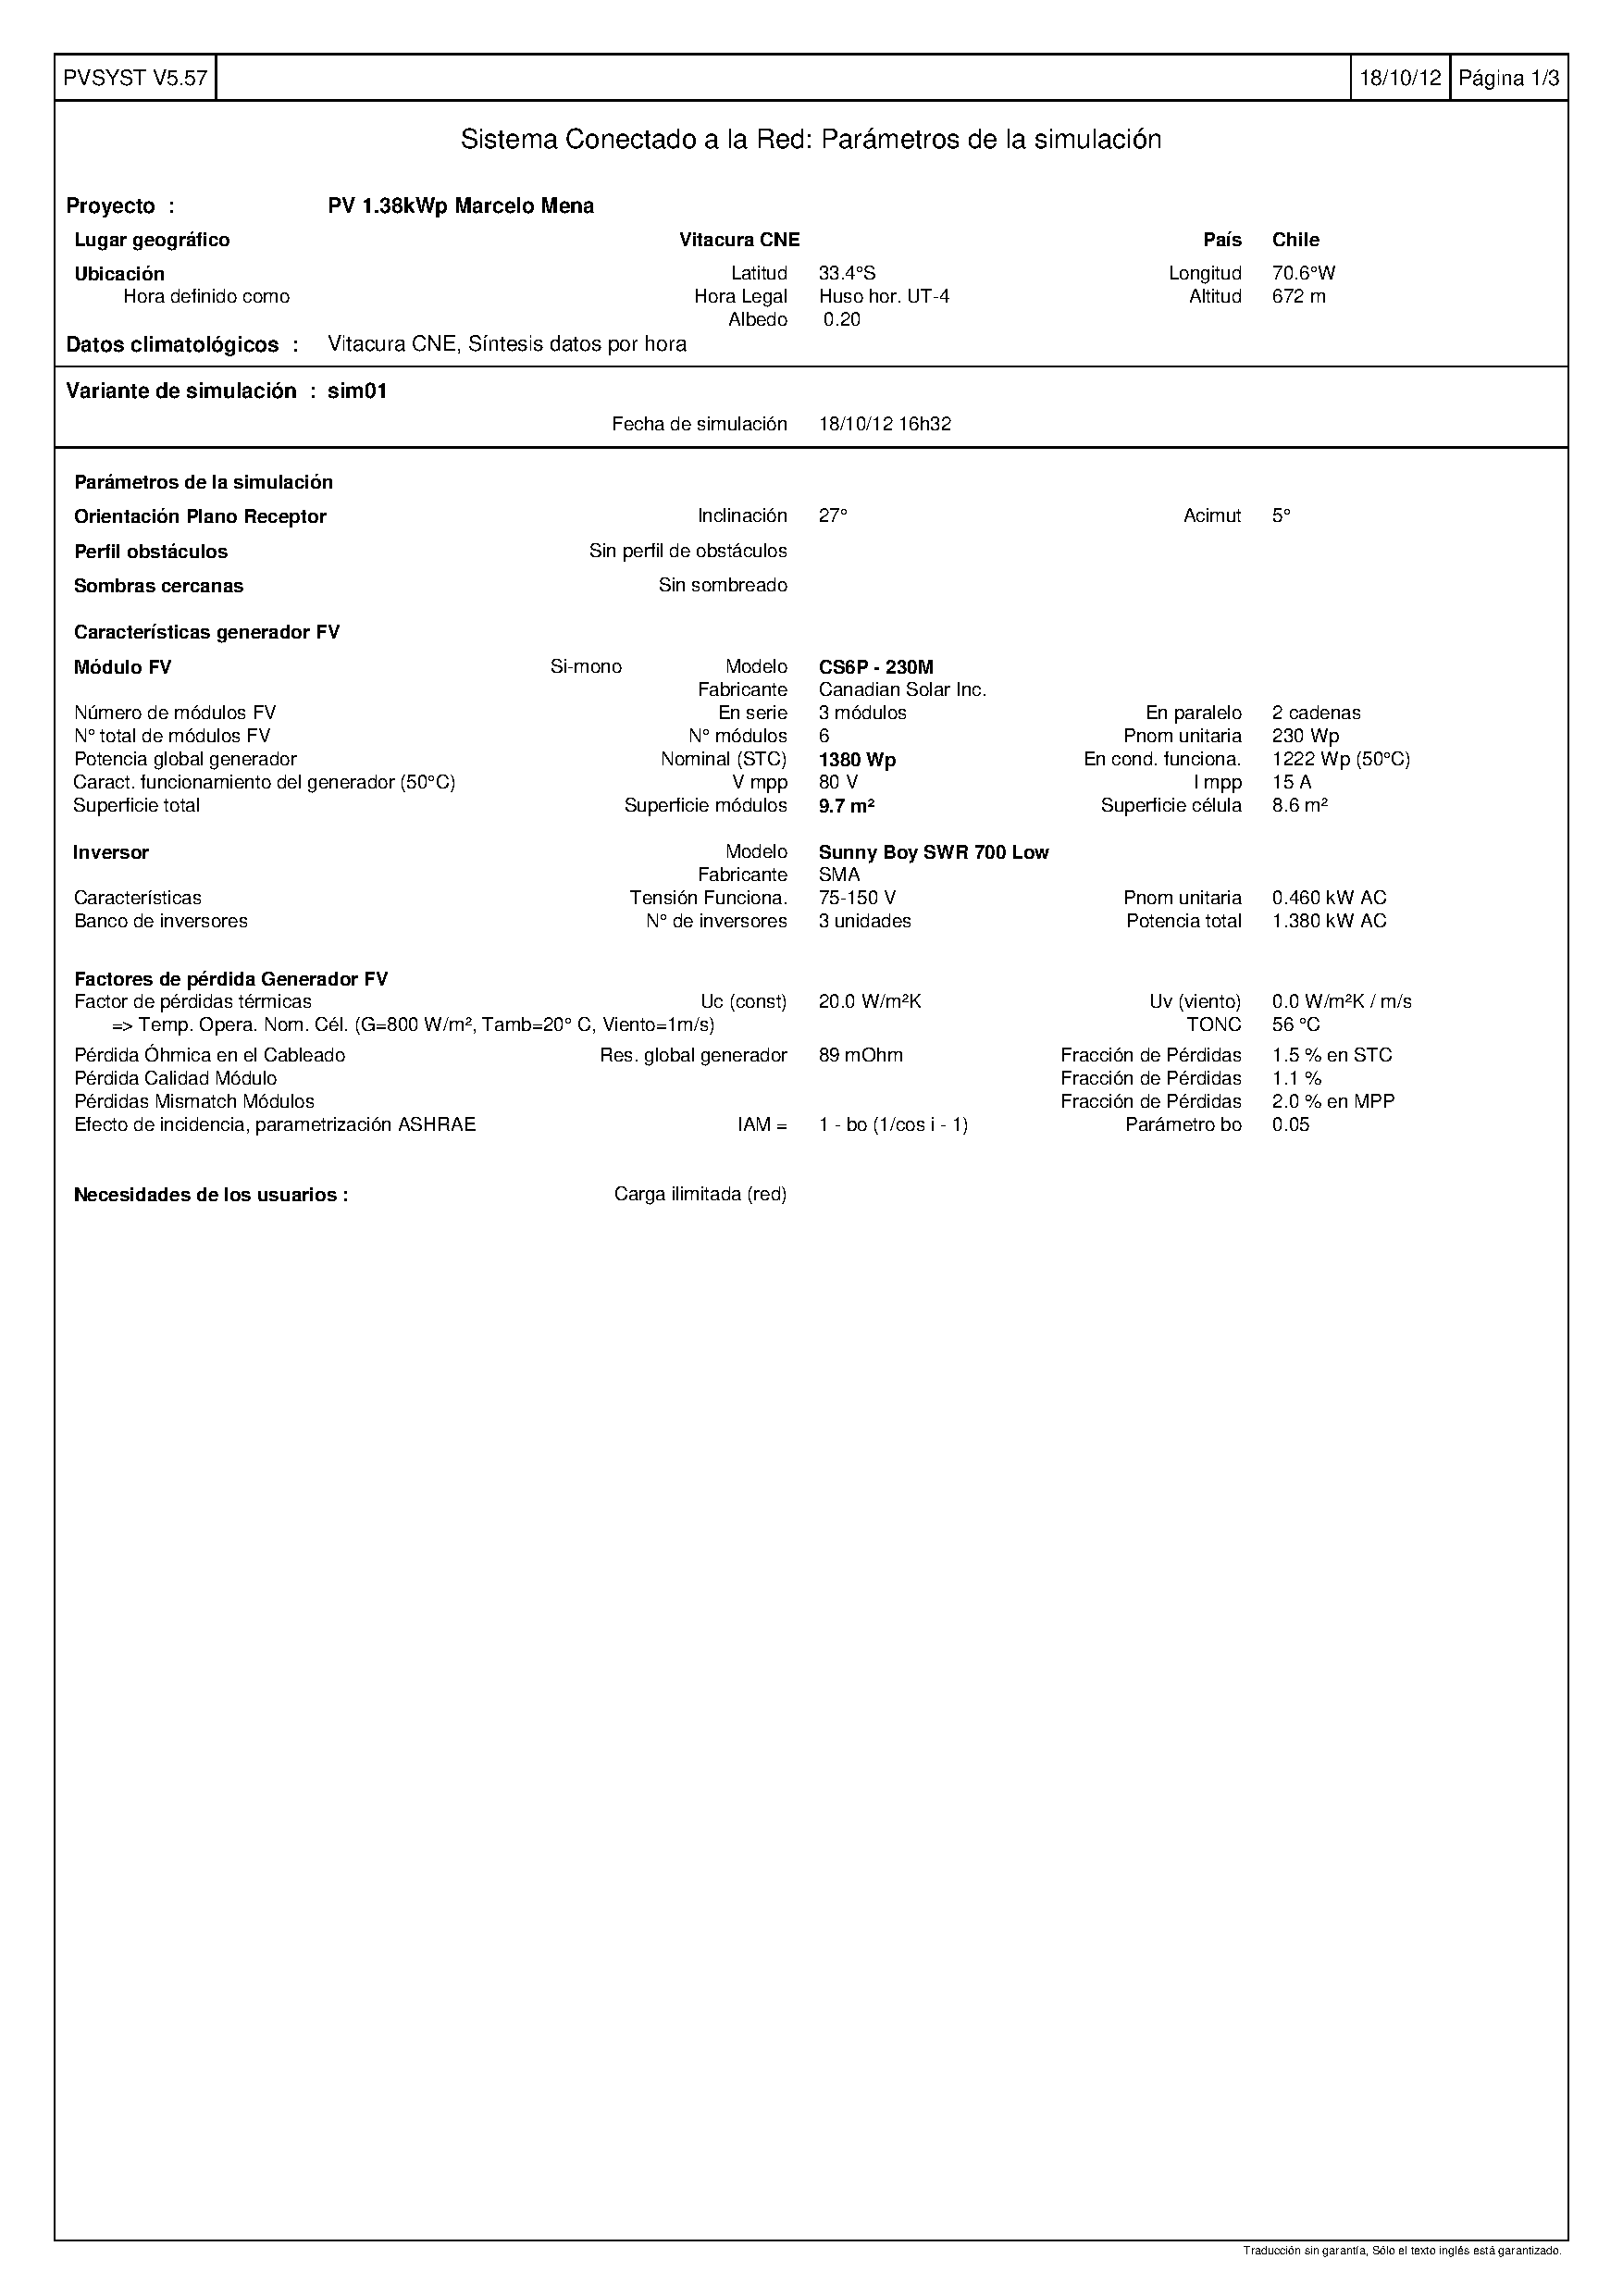
\includepdf[scale=0.85,pages={1},offset=3cm 0cm,pagecommand={\section{Simulación PVSist planta Marcelo Mena}\label{simpvsistmm}\thispagestyle{empty}}]{include/pvsistSim}
\includepdf[scale=0.85,pages={2-3},offset=3cm -1cm]{include/pvsistSim}

\newpage
\label{solarCalcMmena}
\section{Resultados simulacion SolarCalc para planta solar Marcelo Mena}
\label{mmena}

\begin{figure}[h!]
        \centering
        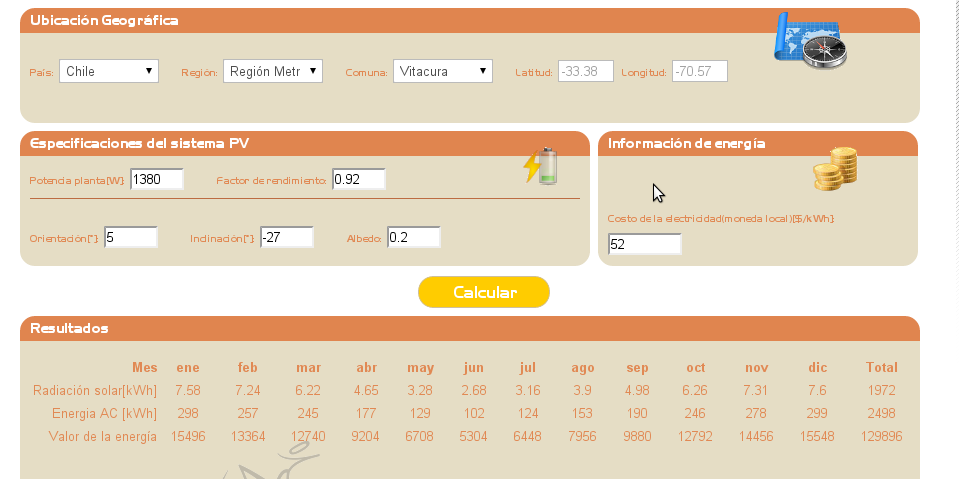
\includegraphics[scale=0.4]{images/simMmena1}
        \caption{Parametros planta solar Marcelo Mena.}
        \label{fotoEstacionFch}
\end{figure}
\begin{figure}[h!]
        \centering
        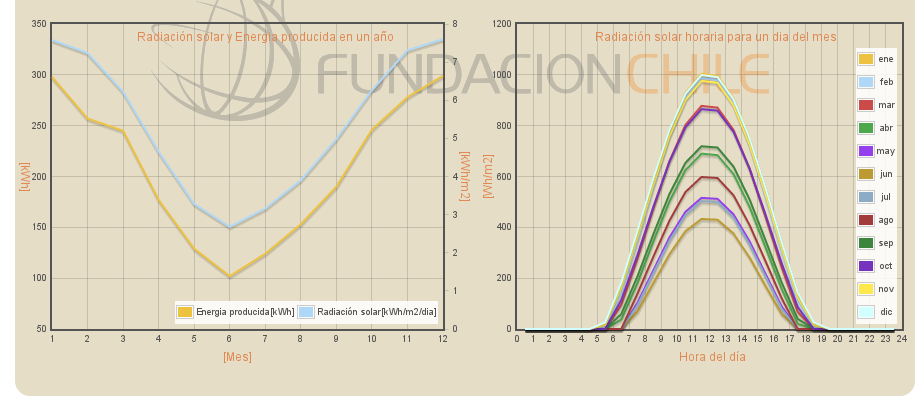
\includegraphics[scale=0.4]{images/simMmena2}
	\caption{Resultados simulacion planta solar Marcelo Mena.}
        \label{fotoEstacionFch}
\end{figure}


\newpage
\label{phpCalculadora}
\subsection{Script implementacion solarCalc}
\label{phpCalculadora}
\begin{verbatim}
<?php
error_reporting(0);
//sleep(1);
/* Calcular la radiacion sobre el plano horizontal horaria a partir de la raciacion diaria de media mensual */
/*BD*/
$datosConexion = array(
        'servidorBD' => "solar.db.7367634.hostedresource.com",
        'usuario' => "widgetSolar",
        'pass' => "corbet*Mount54",
        'bd' => "solar"
        );

$conexion = mysql_connect($datosConexion['servidorBD'], $datosConexion['usuario'], $datosConexion['pass']);
mysql_select_db($datosConexion['bd'], $conexion);

/* Definicion de Constantes */
/*Mes del año*/
$ma = array("ene","feb","mar","abr","may","jun","jul","ago","sep","oct","nov","dic");
/*Numero de dia del año, mitad de mes*/
$nda = array(17,47,75,105,135,162,198,228,258,288,318,344);
/*Numero de disa del mes*/
$ndm = array(31,28,31,30,31,30,31,31,30,31,30,31);
/*Horas del dia */
$hd = array(0.5,1.5,2.5,3.5,4.5,5.5,6.5,7.5,8.5,9.5,10.5,11.5,12.5,13.5,14.5,15.5,16.5,17.5,18.5,19.5,20.5,21.5,22.5,23.5);
/*Constante solar*/
$cs = 1353;

/* Definicion de datos que dependen de la comuna a calcular */
/*Comuna*/
$comuna = utf8_decode($_POST["comuna"]);
/*Consultar BD*/
$q = "SELECT * FROM ene_wh_dia WHERE comuna='".$comuna."'";
$r = mysql_query($q, $conexion) or die(mysql_error());
$RGHd = mysql_fetch_row($r);

$q = "SELECT latitud FROM comunas WHERE comuna='".$comuna."'";
$r = mysql_query($q, $conexion) or die(mysql_error());
$l = mysql_fetch_row($r); $l = $l[0];
 
/*Latitud*/
//$l = -23.3;
/*Radiacion solar global Horizontal diaria de media mensual*/
//$RGHd = $fila;

/*Datos ingresados por el usuario*/
/*Oientacion*/
$ori = $_POST["ori"];
/*Inclinacion*/
$incl = $_POST["incl"];
/*Albedo*/
$alb = $_POST["alb"];
/*potencia peak del panel [W/m2]*/
$ppp = 114.2857;
/*Potencia nominal planta [W]*/
$pnp = $_POST["pnp"];
/*eficiencia del panel*/
$eps = $ppp / 1000;
/*area de la planta*/
$ap = $pnp / $ppp;
/*factor de planta*/
$fp = $_POST["fp"];
/*valor kwh*/
$vkwh = $_POST["vkwh"];

/*Ecuaciones de calculo*/
/*Angulo del dia [rad]*/
function gamma($nda){
	$gamma = ( 2 * M_PI * ($nda - 1) ) / 365;
	return $gamma;
}
/*Declinacion solar*/
function delta($nda){
	$delta = ( (180/M_PI) * (0.006918 - (0.399912*cos(gamma($nda))) + (0.070257*sin(gamma($nda))) - (0.006758*cos(2*gamma($nda))) + (0.000907*sin(2*gamma($nda))) - (0.002697*cos(3*gamma($nda))) + (0.00148*sin(3*gamma($nda))) ) );
	return $delta;
}
/*Angulo de puesta de sol*/
function ws($l,$nda){
	$ws = ( acos( -tan(($l * M_PI) / 180) * tan((delta($nda) * M_PI) / 180) ) * (180/M_PI) );
	return $ws;
}
/*Radiacion solar extraterrestre, estimada a partir del indice de nuvocidad [Wh/m2 dia]*/
function rse($l,$nda,$cs){
	$rse = ( (24 / M_PI) * $cs * (1 + 0.033 * cos(360 * ($nda/365) * (M_PI/180))) * (cos($l * M_PI / 180)) * (cos(delta($nda) * M_PI / 180)) * (sin(ws($l,$nda) * M_PI / 180) - (M_PI / 180 * ws($l,$nda) * cos(ws($l,$nda) * M_PI / 180))));
	return $rse;
}
/*Indice nubosidad [Wh/m2 dia]*/
function kt($RGHd,$l,$nda,$cs){
	$kt = $RGHd / rse($l,$nda,$cs);
	return $kt;
}
/*Horas de sol al dia*/
function hsd($l,$nda){
	$hsd = ws($l,$nda) / 15 * 2 ;
	return $hsd;
}
/*Radiacion solar difusa horizontal diaria de media mensual, a partir de modelo gopinathan KK y soler A, 1995*/
function RDHd($RGHd,$l,$nda,$cs){
	$RDHd = $RGHd * (0.91138 - (0.96225 * kt($RGHd,$l,$nda,$cs)));
	return $RDHd;
}
/*factor a*/
function a($l,$nda){
	$a = (0.409 + (0.5016 * sin((ws($l,$nda) - 60) * M_PI / 180)));
	return $a;
}
/*factor b*/
function b($l,$nda){
	$b = (0.6609 - (0.4767 * sin((ws($l,$nda) - 60) * M_PI / 180)));
        return $b;
}

/*Funciones para calcular algunos datos geometricos*/
function w($hd){
	$w = 15 * ($hd - 12);
	return $w;
}
/*Altura solar*/
function hs($l,$nda,$hd){
	$hs = (asin((sin($l * M_PI / 180) * sin(delta($nda) * M_PI / 180)) + (cos($l * M_PI / 180) * cos(delta($nda) * M_PI / 180) * cos(w($hd) * M_PI / 180))) * (180 / M_PI));
	return $hs;
}
/*Acimut*/
function acimut($l,$nda,$hd){
	$acimut = (acos(( (cos(delta($nda) * M_PI / 180) * cos(w($hd) * M_PI / 180)) - (cos($l * M_PI / 180) * sin(hs($l,$nda,$hd) * M_PI / 180)) ) / (cos(hs($l,$nda,$hd) * M_PI / 180) * sin($l * M_PI / 180))) * 180 / M_PI);
	return ($hd < 12) ? (-1 * $acimut) : $acimut;
}	 

/* Funciones para calcular la distribucion horaria de la radiacion a partir de la radiacion diaria de media mensual */
/*Factor radiacion global horizontal hora/dia*/
function FRGHhd($l,$nda,$hd){
	$FRGHhd = (abs((M_PI / 24) * (a($l,$nda) + (b($l,$nda) * cos(w($hd) * M_PI / 180))) * ((cos(w($hd) * M_PI / 180) - cos(ws($l,$nda) * M_PI / 180))) / (sin(ws($l,$nda) * M_PI / 180) - ((M_PI / 180) * (ws($l,$nda)) * cos(ws($l,$nda) * M_PI / 180)))));
	return $FRGHhd;
}
/*Factor radiacion difusa horizontal hora/dia*/
function FRDfHhd($l,$nda,$hd){
	$FRDfHhd = ((M_PI / 24) * (cos(w($hd) * M_PI / 180) - cos(ws($l,$nda) * M_PI / 180)) / (sin(ws($l,$nda) * M_PI / 180) - (M_PI / 180 * ws($l,$nda) * cos(ws($l,$nda) * M_PI / 180))));
	return $FRDfHhd;
}
/*Radiacion global horaria horizontal*/
function RGHh($RGHd,$l,$nda,$hd){
	if(hs($l,$nda,$hd) > 0){ $RGHh = ($RGHd * FRGHhd($l,$nda,$hd)); }else{ $RGHh = 0;}
	return $RGHh;
}
/*Radiacion difusa horaria horizontal*/
function RDfHh($RGHd,$l,$nda,$cs,$hd){
	if(hs($l,$nda,$hd) > 0){ $RDfHh = (RDHd($RGHd,$l,$nda,$cs) * FRDfHhd($l,$nda,$hd)); }else{ $RDfHh = 0; }
        return $RDfHh;
}
/*Radiacion directa horaria horizontal*/
function RDrHh($RGHd,$l,$nda,$cs,$hd){
	$RDrHh = RGHh($RGHd,$l,$nda,$hd) - RDfHh($RGHd,$l,$nda,$cs,$hd);
	return $RDrHh;
}

/* Funciones para calcular la influencia de la orientacion, inclinacion y refleccion a partir de la radiacion horaria horizontal de media diaria*/
/*Difrencia del angulo con el azimut*/
function difAzimut($ori,$l,$nda,$hd){
	return ($ori - acimut($l,$nda,$hd));
}
/*Angulo horizontal*/
function anguloHorizontal($ori,$l,$nda,$hd){
	return ( ( -1 * $ori ) + acimut($l,$nda,$hd) );
}
/*Angulo vertical*/
function anguloVertical($ori,$RGHd,$l,$nda,$hd){
	$AH = anguloHorizontal($ori,$l,$nda,$hd);
	$HS = hs($l,$nda,$hd);
	if( abs($AH) > 90 ){ 
		$anguloVertical = 90; 
	}else{ 
		if( $HS > 0 ) {
			$anguloVertical = (180 / M_PI * atan(tan($HS * M_PI / 180 ) / cos($AH * M_PI / 180)));
		} else { 
			$anguloVertical = 90;
		}
	}
	return $anguloVertical;
}
/*Angulo de incidencia*/
function anguloIncidencia($incl,$ori,$RGHd,$l,$nda,$hd){
        $HS = hs($l,$nda,$hd);
	$DA = difAzimut($ori,$l,$nda,$hd);
	$anguloIncidencia = (180 / M_PI) * acos( cos($HS * M_PI / 180) * cos($DA * M_PI / 180) * sin($incl * M_PI / 180) + sin($HS * M_PI / 180) * cos($incl * M_PI / 180) );
	return $anguloIncidencia;
}
/*Radiacion directa horaria en la superficie orientada */
function RDrhS($incl,$ori,$RGHd,$l,$nda,$cs,$hd){
	$AI = anguloIncidencia($incl,$ori,$RGHd,$l,$nda,$hd);
	$RDrHh = RDrHh($RGHd,$l,$nda,$cs,$hd);
	$HS = hs($l,$nda,$hd);
	if($AI < 90){ $RDrhS = $RDrHh / sin($HS * M_PI / 180) * cos($AI * M_PI / 180); }else{ $RDrhS = 0;}
	return round($RDrhS);
}
/*Radiacion difuza horaria en la superficie orientada*/
function RDfhS($alb,$incl,$ori,$RGHd,$l,$nda,$cs,$hd){
	$RDfhS = ((1 + cos($incl * M_PI / 180)) / 2 * RDfHh($RGHd,$l,$nda,$cs,$hd)) + (($alb * (1 - cos($incl * M_PI / 180))) / 2 * RGHh($RGHd,$l,$nda,$hd));
	return round($RDfhS);
}
/*Radiacion global horaria den la superficie orientada*/
function RGhS($alb,$incl,$ori,$RGHd,$l,$nda,$cs,$hd){
	$RGhS = (RDrhS($incl,$ori,$RGHd,$l,$nda,$cs,$hd) + RDfhS($alb,$incl,$ori,$RGHd,$l,$nda,$cs,$hd));
	return round($RGhS);
}

/* Energia total solar al mes [Wh/mes]*/
function energiaSolarTotal($alb,$incl,$ori,$RGHd,$l,$nda,$cs,$hd){
	foreach($hd as $var) $energiaSolarT = $energiaSolarT + RGhS($alb,$incl,$ori,$RGHd,$l,$nda,$cs,$var);
	return $energiaSolarT;
}
/* Energia total producida en el mes por la planta [Wh/mes]*/
function energiaProducida($ap,$ep,$fp,$et,$nda){
	$energiaTotal = round($et * $ap * $ep * $fp * $nda);
	return $energiaTotal;
}

/* Realizar los calculos y mostrar el resultado */
/*iterar para todos los meses del año*/

//$filaMes = '<th id=col1 >Mes</th>';
//$filaRadiacion = '<td id=col1>Radiación solar[kWh/m2/dia]</td>';
//$filaEnergia = '<td id=col1>Energia AC [kWh]</td>';
//$filaCosto = '<td id=col1>Valor de la energía</td>';
for($i = 0; $i < 12; $i++){
	$energiaSolarT = round(energiaSolarTotal($alb,$incl,$ori,$RGHd[$i+1],$l,$nda[$i],$cs,$hd) / 1000,2);
	$energiaProducida = energiaProducida($ap,$eps,$fp,$energiaSolarT,$ndm[$i]);
	$energiaValor = round($energiaProducida * $vkwh,2);
	$radiacionHora = array();
	foreach($hd as $var) $radiacionHora[] = array($var,RGhS($alb,$incl,$ori,$RGHd[$i+1],$l,$nda[$i],$cs,$var));

	$r = $r + ($energiaSolarT * $ndm[$i]) ;
	$e = $e + $energiaProducida;
	$c = $c + $energiaValor;

	$filaRadiacion[] = array($i+1,$energiaSolarT);
	$filaEnergia[] = array($i+1,$energiaProducida);
	$filaMes[] = array($i,$ma[$i]);
	$filaCosto[] = array($i,$energiaValor);
	$filaRadiacionHora[] = array('label' => $ma[$i], "data" => $radiacionHora, 'color' => $i); 
}

/* Codificar los datos en JSON */
$r = round($r,0);
$e = round($e,0);
$c = round($c,2);
$datos = array(
	array('label' => 'Energia producida[kWh]', "data" => $filaEnergia, 'yaxis' => 1),
	array('label' => 'Radiación solar[kWh/m2/dia]', "data" => $filaRadiacion, 'yaxis' => 2),
	array('label' => 'meses', "data" => $filaMes, 'yaxis' => 3),
	array('label' => 'costo', "data" => $filaCosto, 'yaxis' => 4),
	array('label' => 'totalR', "data" => $r, 'yaxis' => 5),
	array('label' => 'totalE', "data" => $e, 'yaxis' => 5),
	array('label' => 'totalC', "data" => $c, 'yaxis' => 5),
);
$datos = array_merge($datos,$filaRadiacionHora);

	header('Content-type: application/json');
$datos = json_encode($datos);
echo $datos;
?>
\end{verbatim}


\newpage
\label{getData}
\section{Script CRBasic - Datalogger estación Fundación Chile}
\label{getData}
\begin{verbatim}
'CR800
'Manuel Arredondo for CR800 Estación FCH Vitacura
'29/08/2012

'Declare Variables and Units
Public BattV
Public ApogeeFCH
Public SlrMJ
Public AirTC
Public RH

Public PTemp, batt_volt
Public socket, serial
Public GetRequest As String * 200
Public GetResponse As String * 200
Public httpGetMsg As String * 200
Public ipServer As String *200
Public varsGetRequest As String * 600

Units BattV=Volts
Units ApogeeFCH=W/m^2
Units SlrMJ=MJ/m^2
Units AirTC=Deg C
Units RH=%

'Define Data Tables
DataTable(solarFch,True,-1)
	DataInterval(0,1,Min,10)
	Sample(1,BattV,FP2)
	Sample(1,ApogeeFCH,FP2)
	Totalize(1,SlrMJ,IEEE4,False)
	Sample(1,AirTC,FP2)
	Sample(1,RH,FP2)
EndTable

'Main Program
BeginProg
	Scan(1,Min,1,0)
		'Def timestamp
		'TimeS = Status.timestamp(1,1)
		'TimeS = solarFch.TimeStamp

		'Default Datalogger Battery Voltage measurement BattV
		Battery(BattV)

		'Apogee Pyranometer measurements SlrMJ and ApogeeFCH
		VoltDiff(ApogeeFCH,1,mV250,1,True,0,_50Hz,1,0)
		If ApogeeFCH<0 Then ApogeeFCH=0
		SlrMJ=ApogeeFCH*0.012
		ApogeeFCH= ApogeeFCH*5.41

		'HMP50 Temperature & Relative Humidity Sensor measurements AirTC
		'and RH

		VoltSe(AirTC,1,mV2500,3,0,0,_50Hz,0.1,-40)
		VoltSe(RH,1,mV2500,4,0,0,_50Hz,0.1,0)
		If (RH>100) AND (RH<108) Then RH=100
		
		'Call Data Tables and Store Data
		CallTable(solarFch)

		'peticion get al servidor de solaratacama.cl para registrar las
		'lecturas en la BD

		ipServer = "www.solaratacama.cl"
		'varsGetRequest = "timestamp="+TimeS+"&battV="+BattV+"&radW="+
		Rad_W+"&radW2="+Rad_W_2+"&airTc="+AirTC+"&rh="+RH

		varsGetRequest = "battV="+BattV+"&radW="+ApogeeFCH+"&radW2="+
		SlrMJ+"&airTc="+AirTC+"&rh="+RH    
		GetRequest = "GET /solarDatos/getDatalogerFch.php?"+varsGetRequest+
		" HTTP/1.1"+CHR(13)+CHR(10)
		'GetRequest = "GET /getDatalogerFch.php HTTP/1.1"+CHR(13)+CHR(10)
		socket = TCPOpen(ipServer,80,1024)
		serial = SerialOpen(ComRS232,9600,0,20000,1000)
		if socket <> 0 Then
			SerialOut(socket,GetRequest,"",0,0)
			SerialOut(socket,"User-Agent:Mozilla/5.0"+CHR(13)+CHR(10),"",0,0)
			SerialOut(socket,"Host:"+ipServer+CHR(13)+CHR(10),"",0,0)
			SerialOut(socket,CHR(13)+CHR(10),"",0,0)
			SerialOut(serial,GetRequest,"0",1,150)
			SerialIn(GetResponse,socket,500,"",200)
			SerialOut(serial,GetResponse,"0",1,150)
		EndIf
	NextScan
EndProg
\end{verbatim}




%\footbibliographystyle{plain}
%\footbibliography{include/bibliografia}
%\bibliographystyle{plain}
%\bibliography{include/bibliografia}
\printbibliography[title=Bibliografia] %(5)

\end{document}
